\documentclass[oneside,openany,phd]{TMU-Thesis}


% ==================== structure/preamble.tex ====================
% مشخصات پایان‌نامه را در فایلهای faTitle و enTitle وارد نمایید.
% در اینجا برای یکپارچگی، همینجا وارد می‌کنیم

% مشخصات فارسی
\university{تربیت مدرس}
\faculty{مهندسی برق و کامپیوتر}
\department{گروه هوش مصنوعی و رباتیکز}
\subject{مهندسی کامپیوتر}
\field{مهندسی نرم‌افزار}
\credits{---} % در رساله دکتری معمولا به صورت واحدی ذکر نمی‌شود یا فیلد خالی است
\title{یادگیری تقویتی عمیق با شکل‌دهی تصادفی پاداش برای مدیریت عدم قطعیت در سیستم‌های خودوفقی}
\firstsupervisor{دکتر ...}
% \secondsupervisor{استاد راهنمای دوم}
\firstadvisor{دکتر ...}
% \secondadvisor{استاد مشاور دوم}
\name{علیرضا}
\surname{کاویانی‌فر}
\studentID{...}
\thesisdate{بهمن ۱۴۰۴}

% مشخصات انگلیسی
\latinuniversity{Tarbiat Modares University}
\latinfaculty{Faculty of Electrical and Computer Engineering}
\latinsubject{Computer Engineering}
\latinfield{Software Engineering}
\latintitle{Randomized Reward-Shaped Deep Reinforcement Learning for Managing Uncertainty in Self-Adaptive Systems}
\firstlatinsupervisor{Dr. ...}
\firstlatinadvisor{Dr. ...}
\latinname{Alireza}
\latinsurname{Kavianifar}
\latinthesisdate{February 2026}
\latinkeywords{Self-Adaptive Systems, Deep Reinforcement Learning, Randomized Reward Shaping, Uncertainty Management, Formal Verification, UPPAAL-SMC}

% فراخوانی بسته‌ها و دستورات استاندارد
% در این فایل، دستورها و تنظیمات مورد نیاز، آورده شده است.
%-------------------------------------------------------------------------------------------------------------------

% در ورژن جدید زی‌پرشین برای تایپ متن‌های ریاضی، این سه بسته، حتماً باید فراخوانی شود
\usepackage{amsthm,amssymb,amsmath}
% بسته‌ای برای تنطیم حاشیه‌های بالا، پایین، چپ و راست صفحه
\usepackage[top=30mm, bottom=25mm, left=25mm, right=35mm]{geometry}
% بسته‌‌ای برای ظاهر شدن شکل‌ها و تصاویر متن
\usepackage{graphicx}
% بسته‌ای برای رسم کادر
\usepackage{framed} 
% بسته‌‌ای برای چاپ شدن خودکار تعداد صفحات در صفحه «معرفی پایان‌نامه»
\usepackage{lastpage}
% بسته‌ و دستوراتی برای ایجاد لینک‌های رنگی با امکان جهش
% \usepackage[pagebackref=false,colorlinks,linkcolor=black,citecolor=black]{hyperref}
% چنانچه قصد پرینت گرفتن نوشته خود را دارید، خط بالا را غیرفعال و  از دستور زیر استفاده کنید چون در صورت استفاده از دستور زیر‌‌، 
% لینک‌ها به رنگ سیاه ظاهر خواهند شد که برای پرینت گرفتن، مناسب‌تر است
% \usepackage[pagebackref=false]{hyperref}
% بسته‌ لازم برای تنظیم سربرگ‌ها
\usepackage{fancyhdr}
\setlength{\headheight}{16pt}
%
\usepackage{setspace}
\usepackage{algorithm}
\usepackage{algorithmic}
\usepackage{subfigure}
\usepackage[subfigure]{tocloft}
\usepackage{multirow}


% بسته‌ای برای ظاهر شدن «مراجع» و «نمایه» در فهرست مطالب
\usepackage[nottoc]{tocbibind}
% دستورات مربوط به ایجاد نمایه
\usepackage{makeidx}
\makeindex
% تعریف شیم‌های مورد نیاز برای نسخه‌های جدید بسته bidi در برخی محیط‌ها
% Removal of redundant and potentially broken definitions
\makeatletter
% شیم‌های سازگاری برای نسخه‌های جدید لاتک و بسته‌های bidi/xepersian
\providecommand{\IfClassLoadedT}[2]{\@ifclassloaded{#1}{#2}{}}
\providecommand{\IfClassLoadedF}[2]{\@ifclassloaded{#1}{}{#2}}
\providecommand{\IfClassLoadedTF}[3]{\@ifclassloaded{#1}{#2}{#3}}
\providecommand{\IfPackageLoadedT}[2]{\@ifpackageloaded{#1}{#2}{}}
\providecommand{\IfPackageLoadedF}[2]{\@ifpackageloaded{#1}{}{#2}}
\providecommand{\IfPackageLoadedTF}[3]{\@ifpackageloaded{#1}{#2}{#3}}
\providecommand{\@iffileloaded}[3]{\expandafter\ifx\csname ver@#1\endcsname\relax#3\else#2\fi}
\providecommand{\IfFileLoadedT}[2]{\@iffileloaded{#1}{#2}{}}
\providecommand{\IfFileLoadedF}[2]{\@iffileloaded{#1}{}{#2}}
\providecommand{\IfFileLoadedTF}[3]{\@iffileloaded{#1}{#2}{#3}}
\makeatother

%%%%%%%%%%%%%%%%%%%%%%%%%%
% فراخوانی بسته زی‌پرشین و تعریف قلم فارسی و انگلیسی
\usepackage[pagebackref=false,colorlinks,linkcolor=black,citecolor=black]{hyperref}
\usepackage{notoccite}

\ExplSyntaxOn
\cs_if_exist:NTF \g__hyp_linknestlevel_int { } { \int_new:N \g__hyp_linknestlevel_int }
\cs_if_exist:NTF \l__hyp_annot_GoTo_bool { } { \bool_new:N \l__hyp_annot_GoTo_bool }
\cs_if_exist:NTF \l__hyp_annot_URI_bool { } { \bool_new:N \l__hyp_annot_URI_bool }
\cs_if_exist:NTF \l__hyp_href_url_ismap_bool { } { \bool_new:N \l__hyp_href_url_ismap_bool }
\cs_if_exist:NTF \l__hyp_text_enc_uri_print_tl { } { \tl_new:N \l__hyp_text_enc_uri_print_tl }
\cs_if_exist:NTF \l__hyp_uri_tmpa_tl { } { \tl_new:N \l__hyp_uri_tmpa_tl }

% Defining missing l3pdf/pdfdict commands if not present
\cs_if_exist:NTF \pdfdict_put:nno { } { \cs_new:Npn \pdfdict_put:nno #1#2#3 { } }
\cs_if_exist:NTF \pdfdict_put:nnn { } { \cs_new:Npn \pdfdict_put:nnn #1#2#3 { } }
\cs_if_exist:NTF \pdfdict_use:n { } { \cs_new:Npn \pdfdict_use:n #1 { } }
\cs_if_exist:NTF \pdfannot_dict_put:nne { } { \cs_new:Npn \pdfannot_dict_put:nne #1#2#3 { } }
\cs_if_exist:NTF \pdfannot_link:nen { } { \cs_new:Npn \pdfannot_link:nen #1#2#3 { } }
\cs_if_exist:NTF \__hyp_check_link_nesting:TF { } { \cs_new:Npn \__hyp_check_link_nesting:TF #1#2 { #1 } }
\cs_if_exist:NTF \__hyp_text_pdfstring:eoN { } { \cs_new:Npn \__hyp_text_pdfstring:eoN #1#2#3 { } }
\ExplSyntaxOff

% تعریف دستورات گمشده برای جلوگیری از خطای renewcommand در بسته‌های داخلی
\makeatletter
\providecommand{\foottextfont}{}
\providecommand{\LTRfoottextfont}{}
\providecommand{\RTLfoottextfont}{}
\providecommand{\abstractname}{}
\providecommand{\latinabstract}{}
\providecommand{\AutoPersianDigits}{}
\makeatother

\usepackage{xepersian}
\settextfont[Path=font/,Extension=.ttf,Scale=1,
    BoldFont=XB NiloofarBd,
    ItalicFont=XB NiloofarIt,
    BoldItalicFont=XB NiloofarBdIt
]{XB Niloofar}
\setlatintextfont[Scale=0.9]{Times New Roman}

%%%%%%%%%%%%%%%%%%%%%%%%%%
% چنانچه می‌خواهید اعداد در فرمول‌ها، انگلیسی باشد، خط زیر را غیرفعال کنید
\setdigitfont[Path=font/,Extension=.ttf,Scale=1,
    BoldFont=XB NiloofarBd,
    ItalicFont=XB NiloofarIt,
    BoldItalicFont=XB NiloofarBdIt
]{XB Niloofar}
%%%%%%%%%%%%%%%%%%%%%%%%%%
% تعریف قلم‌های فارسی و انگلیسی اضافی برای استفاده در بعضی از قسمت‌های متن
\defpersianfont\titlefont[Path=font/,Extension=.ttf,Scale=1]{XB Titre}
% \defpersianfont\iranic[Scale=1.1]{XB Zar Oblique}%Italic}%
% \defpersianfont\nastaliq[Scale=1.2]{IranNastaliq}

%%%%%%%%%%%%%%%%%%%%%%%%%%
% دستوری برای حذف کلمه «چکیده»
\renewcommand{\abstractname}{}
% دستوری برای حذف کلمه «abstract»
%\renewcommand{\latinabstract}{}
% دستوری برای تغییر نام کلمه «اثبات» به «برهان»
\renewcommand\proofname{\textbf{برهان}}
% دستوری برای تغییر نام کلمه «کتاب‌نامه» به «مراجع»
\renewcommand{\bibname}{مراجع}
% دستوری برای تعریف واژه‌نامه انگلیسی به فارسی
\newcommand\persiangloss[2]{#1\dotfill\lr{#2}\\}
% دستوری برای تعریف واژه‌نامه فارسی به انگلیسی 
\newcommand\englishgloss[2]{#2\dotfill\lr{#1}\\}
% تعریف دستور جدید «\پ» برای خلاصه‌نویسی جهت نوشتن عبارت «پروژه/پایان‌نامه/رساله»
\newcommand{\پ}{پروژه/پایان‌نامه/رساله }

%\newcommand\BackSlash{\char`\\}

%%%%%%%%%%%%%%%%%%%%%%%%%%
\SepMark{-}

% تعریف و نحوه ظاهر شدن عنوان قضیه‌ها، تعریف‌ها، مثال‌ها و ...
\theoremstyle{definition}
\newtheorem{definition}{تعریف}[section]
\theoremstyle{plain}
\newtheorem{theorem}[definition]{قضیه}
\newtheorem{lemma}[definition]{لم}
\newtheorem{proposition}[definition]{گزاره}
\newtheorem{corollary}[definition]{نتیجه}
\newtheorem{remark}[definition]{ملاحظه}
\theoremstyle{definition}
\newtheorem{example}[definition]{مثال}

%\renewcommand{\theequation}{\thechapter-\arabic{equation}}
%\def\bibname{مراجع}
\numberwithin{algorithm}{chapter}
\def\listalgorithmname{فهرست الگوریتم‌ها}
\def\listfigurename{فهرست تصاویر}
\def\listtablename{فهرست جداول}

%%%%%%%%%%%%%%%%%%%%%%%%%%%%
% دستورهایی برای سفارشی کردن سربرگ صفحات
% \newcommand{\SetHeader}{
% \csname@twosidetrue\endcsname
% \pagestyle{fancy}
% \fancyhf{} 
% \fancyhead[OL,EL]{\thepage}
% \fancyhead[OR]{\small\rightmark}
% \fancyhead[ER]{\small\leftmark}
% \renewcommand{\chaptermark}[1]{%
% \markboth{\thechapter-\ #1}{}}
% }
%%%%%%%%%%%%5
%\def\MATtextbaseline{1.5}
%\renewcommand{\baselinestretch}{\MATtextbaseline}
\doublespacing
%%%%%%%%%%%%%%%%%%%%%%%%%%%%%
% دستوراتی برای اضافه کردن کلمه «فصل» و شماره ترتیبی حروفی در فهرست مطالب

\makeatletter
% سفارشی‌سازی عدد ۱ در سیستم ابجد برای نمایش کلمه «الف» به جای «آ»
\def\@abjad#1{%
\ifnum#1=1 الف%
\else
  \ifnum#1>1999 \xpg@warning{Illegal value (#1) for abjad numeral} {#1}%
  \else
    \ifnum#1<\z@\space\xpg@warning{Illegal value (#1) for abjad numeral}%
    \else
      \ifnum#1<10\expandafter\abj@num@i\number#1%
      \else
        \ifnum#1<100\expandafter\abj@num@ii\number#1%
        \else
          \ifnum#1<\@m\expandafter\abj@num@iii\number#1%
          \else
            \ifnum#1<\@M\expandafter\abj@num@iv\number#1%
            \fi
          \fi
        \fi
      \fi
    \fi
  \fi
\fi}
\def\abj@num@i#1{%
  \ifcase#1\or ا\or ب\or ج\or د%
           \or ه\or و\or ز\or ح\or ط\fi
  \ifnum#1=\z@\abjad@zero\fi}

\newcommand{\persianchapnum}[1]{%
  \edef\@arg{#1}%
  \def\@one{1}\def\@pone{۱}%
  \def\@two{2}\def\@ptwo{۲}%
  \def\@three{3}\def\@pthree{۳}%
  \def\@four{4}\def\@pfour{۴}%
  \def\@five{5}\def\@pfive{۵}%
  \def\@six{6}\def\@psix{۶}%
  \def\@seven{7}\def\@pseven{۷}%
  \def\@eight{8}\def\@peight{۸}%
  \def\@nine{9}\def\@pnine{۹}%
  \def\@ten{10}\def\@pten{۱۰}%
  \ifx\@arg\@one اول%
  \else\ifx\@arg\@pone اول%
  \else\ifx\@arg\@two دوم%
  \else\ifx\@arg\@ptwo دوم%
  \else\ifx\@arg\@three سوم%
  \else\ifx\@arg\@pthree سوم%
  \else\ifx\@arg\@four چهارم%
  \else\ifx\@arg\@pfour چهارم%
  \else\ifx\@arg\@five پنجم%
  \else\ifx\@arg\@pfive پنجم%
  \else\ifx\@arg\@six ششم%
  \else\ifx\@arg\@psix ششم%
  \else\ifx\@arg\@seven هفتم%
  \else\ifx\@arg\@pseven هفتم%
  \else\ifx\@arg\@eight هشتم%
  \else\ifx\@arg\@peight هشتم%
  \else\ifx\@arg\@nine نهم%
  \else\ifx\@arg\@pnine نهم%
  \else\ifx\@arg\@ten دهم%
  \else\ifx\@arg\@pten دهم%
  \else #1\fi\fi\fi\fi\fi\fi\fi\fi\fi\fi\fi\fi\fi\fi\fi\fi\fi\fi\fi\fi
}

\newlength\mylenprt
\newlength\mylenchp
\newlength\mylenapp

\renewcommand\cftpartpresnum{\partname~}
\renewcommand\cftchappresnum{\chaptername~}
\renewcommand\cftchapaftersnum{:}

\settowidth\mylenprt{\cftpartfont\cftpartpresnum\cftpartaftersnum}
% تنظیم پهنای کادر شماره متناسب با عریض‌ترین عنوان فصل («فصل چهارم: »)
\settowidth\mylenchp{\cftchapfont\chaptername~چهارم:\space}
\settowidth\mylenapp{\cftchapfont\appendixname~\cftchapaftersnum}
\addtolength\mylenprt{\cftpartnumwidth}
\addtolength\mylenchp{0.5em}
\addtolength\mylenapp{\cftchapnumwidth}

\setlength\cftpartnumwidth{\mylenprt}
\setlength\cftchapnumwidth{\mylenchp}

% اعمال تبدیل شماره فصل به حروف در فهرست مطالب با رعایت چیدمان راست‌به‌چپ (RTL)
\renewcommand*{\l@chapter}[2]{%
  \ifnum \c@tocdepth >\m@ne
    \addpenalty{-\@highpenalty}%
    \vskip \cftbeforechapskip
    {\if@RTL\rightskip\else\leftskip\fi \cftchapindent\relax
     \if@RTL\leftskip\else\rightskip\fi \@tocrmarg
     \parfillskip -\if@RTL\leftskip\else\rightskip\fi
     \parindent \cftchapindent\relax\@afterindenttrue
     \interlinepenalty\@M
     \leavevmode
     \@tempdima \cftchapnumwidth\relax
     \let\@cftbsnum \cftchappresnum
     \let\@cftasnum \cftchapaftersnum
     \let\@cftasnumb \cftchapaftersnumb
     \advance\if@RTL\rightskip\else\leftskip\fi \@tempdima \null\nobreak\hskip -\if@RTL\rightskip\else\leftskip\fi
     {\cftchapfont \def\numberline##1{\hb@xt@\@tempdima{\@cftbsnum \persianchapnum{##1}\@cftasnum\hfil}\@cftasnumb}#1}\nobreak
     \cftchapfillnum{#2}}%
  \fi}

% فعال‌سازی نقطه‌چین برای فصول در فهرست مطالب هماهنگ با بخش‌ها
\renewcommand{\cftchapleader}{\cftdotfill{\cftsecdotsep}}

% اصلاح نمایش پیوست‌ها در فهرست مطالب (تبدیل «فصل آ» به «پیوست آ»)
\g@addto@macro\appendix{%
  \addtocontents{toc}{%
    \protect\renewcommand{\protect\cftchappresnum}{\protect\appendixname~}%
  }%
}

% اصلاح سرتیتر شروع فصول در متن اصلی به صورت حروف فارسی
\def\@makechapterhead#1{%
  \vspace*{50\p@}%
  {\parindent \z@ \raggedright \normalfont
    \ifnum \c@secnumdepth >\m@ne
      \if@mainmatter
        \huge\bfseries \@chapapp\space 
        \ifx\@chapapp\appendixname
          \thechapter
        \else
          \persianchapnum{\the\c@chapter}
        \fi
        \par\nobreak
        \vskip 20\p@
      \fi
    \fi
    \interlinepenalty\@M
    \Huge \bfseries #1\par\nobreak
    \vskip 40\p@
  }}
\makeatother

\makeatletter
{\def\thebibliography#1{\chapter*{\refname\@mkboth
   {\uppercase{\refname}}{\uppercase{\refname}}}\list
   {[\arabic{enumi}]}{\settowidth\labelwidth{[#1]}
   \rightmargin\labelwidth
   \advance\rightmargin\labelsep
   \advance\rightmargin\bibindent
   \itemindent -\bibindent
   \listparindent \itemindent
   \parsep \z@
   \usecounter{enumi}}
   \def\newblock{}
   \sloppy
   \sfcode`\.=1000\relax}}
\makeatother

% Standalone configuration to support individual chapter compilation
\ifdefined\ifstandalone
\else
  \newif\ifstandalone
  \standalonetrue
\fi


% تنظیمات اختصاصی برای فهرست مطالب (TOC)
\setcounter{secnumdepth}{3}
\setcounter{tocdepth}{3}

\raggedbottom

% تنظیمات نقطه‌چین برای فهرست مطالب
\usepackage{tocloft}
\providecommand{\cftchapdotfill}{\cftdotfill{\cftdotsep}}
\providecommand{\cftsecdotfill}{\cftdotfill{\cftdotsep}}
\providecommand{\cftsubsecdotfill}{\cftdotfill{\cftdotsep}}


% تنظیمات سربرگ برای رفع مشکل نمایش حروف فارسی (جعبه‌های خالی)
\usepackage{fancyhdr}
\pagestyle{fancy}
\fancyhf{}
\fancyhead[L]{\thepage}
\fancyhead[R]{\small\leftmark}
\renewcommand{\chaptermark}[1]{\markboth{\chaptername\ \thechapter.\ #1}{}}
\renewcommand{\sectionmark}[1]{\markright{\thesection.\ #1}}
% حذف حالت ایتالیک/کج که باعث به هم ریختگی فونت فارسی در سربرگ می‌شود
\let\oldheadrule\headrule
\renewcommand{\headrule}{\oldheadrule}
\fancyhead[R]{\small\nouppercase{\leftmark}}



\begin{document}
\AutoPersianDigits
\setstretch{1.5}

\setcounter{chapter}{3}

\chapter{روش پیشنهادی}
\label{ch:chapter4}
\label{ch:methodology}
\label{ch:chapter5-process}

\section{مقدمه}
\label{sec:ch4_intro}

طراحی و توسعه سیستم‌های نرم‌افزاری خودوفق زمان واقعی در محیط‌های پویا و نویزی، مستلزم ایجاد موازنه عمیقی میان دو دغدغه متضاد مهندسی است: تصمیم‌گیری فوق‌سریع در مقیاس میلی‌ثانیه جهت همگامی با تغییرات محیطی، و ارائه تضمین‌های صوری و ریاضیاتی مبتنی بر ایمنی و انطباق کامل با اهداف کیفیت خدمات (\lr{QoS}). همان‌طور که در فصل‌های پیشین تبیین گردید، روش‌های کلاسیک بهینه‌سازی و وارسی مدل آنلاین به دلیل محدودیت شدید مقیاس‌پذیری و زمان‌های محاسباتی طولانی (که در رده مسائل ان‌پی-سخت طبقه‌بندی می‌شوند \cite{garey1979computers, coker2015sass}) قادر به برآوردن این الزامات در مقیاس‌های عملیاتی نیستند.

از سوی دیگر، یادگیری تقویتی عمیق استاندارد (\lr{DRL}) اگرچه زمان تصمیم‌گیری را به شدت کاهش می‌دهد، اما به علت پدیده «تنکی پاداش» (\lr{Reward Sparsity}) \cite{du2023alleviating} و رانش مفهومی \cite{gheibi2024dealing}، در مواجهه با فضاهای پیکربندی بزرگ به نقاط بهینه محلی همگرا گشته و فاقد تضمین‌های صوری زمان اجراست. علاوه بر این، در سیستم‌های فیزیکی-سایبری بلادرنگ با مهلت‌های زمانی سخت (۲۰ تا ۵۰ میلی‌ثانیه) و توزیع داده‌های با غلبه بیش از ۹۰٪ شکست در لاگ‌های بازپخش، روش‌های یادگیری بدون هدایت دچار فروپاشی ارزش شده و سپرهای ایمنی کلاسیک نیز به علت شکاف واقعیت میان مدل‌های جانشین آماری و فیزیک اجرای پرواز، با شکست‌های فاجعه‌بار مواجه می‌گردند.

هدف اصلی این فصل، ارائه جزئیات فنی، معماری و ریاضیاتی روش پیشنهادی رساله در قالب یک ساختار پیش‌رونده دو‌بخشی است:
\begin{itemize}
    \item \textbf{بخش اول: چارچوب پایه‌ای \lr{RS-DRL} برای سیستم‌های توزیع‌شده با کیفیت خدمات نرم:} در این بخش، اصل تفکیک زمانی (\lr{Temporal Separation})، یکپارچه‌سازی ناهمگام با حلقه خودمختار \lr{MAPE-K}، سازوکار شکل‌دهی تصادفی پاداش با پارامتر خوش‌بینی $\rho$ جهت عبور از بهینه‌های محلی، و بازبینی صوری توسط ابزار \lr{UPPAAL-SMC} تشریح می‌گردد.
    \item \textbf{بخش انتقال: چالش‌های فیزیکی-سایبری و سه‌گانه برنامه‌ریزی زمان‌حقیقی:} در این بخش، چرایی ناکارآمدی رویکردهای یکنواخت پیشین در مواجهه با مهلت‌های زمانی ۲۰ تا ۵۰ میلی‌ثانیه، لاگ‌های با بیش از ۹۰٪ شکست، و شکاف واقعیت مدل‌های جانشین مورد تحلیل ریاضی و معماری قرار می‌گیرد.
    \item \textbf{بخش دوم: معماری تعمیم‌یافته \rsdrlplus برای سیستم‌های فیزیکی-سایبری بلادرنگ:} در این بخش، دو الگوی طراحی نرم‌افزاری نوین معرفی می‌شوند:
    \begin{enumerate}
        \item الگوی \textbf{سنتز آفلاین هدایت‌شده با مشخصه‌ها (\sgos)} شامل دو رویکرد \mursdrl (حاشیه بازیابی شکست و مشوق مطلوبیت) و \cmrsdrl (بافرسازی حاشیه اطمینان) جهت پالایش شکست‌های غیرقابل‌جبران و هدایت گرادیان.
        \item الگوی \textbf{اعتبارسنجی کشسان فاز برنامه‌ریزی با قرارداد در هر زمان (\caepv)} در قالب ماژول \pgalr، شامل استنتاج زیر میلی‌ثانیه‌ای، گیت تنش محیطی، و پالایش موضعی ۱-گام مقید به ابعاد حساسیت توضیح‌پذیر \lr{TreeSHAP} همراه با اثبات صوری گزاره ۱ (کران کاردینالیتی $\mathcal{O}(m \cdot K)$) و گزاره ۲ (تضمین ایمنی یکنواخت).
    \end{enumerate}
\end{itemize}

در ادامه، جزئیات هر یک از این بخش‌ها، فرمول‌بندی‌های صوری، الگوریتم‌های اجرایی و نگاشت آن‌ها بر پرسش‌های پژوهش تبیین می‌گردد.

\section{اصول معماری سطح بالا و سازماندهی فرآیند}
\label{sec:ch5-overview}

یک سیستم خودوفق کارآمد در محیط‌های همراه با عدم قطعیت، باید ذاتاً بین دغدغه‌های متضاد طراحی مانند تصمیم‌گیری آنلاین با تأخیر بسیار کم و آموزش سنگین و ناهمگام مدل‌های یادگیری، تفکیک قائل شود تا بتواند آن‌ها را به‌طور مؤثر در یک ریسمان کنترلی واحد مدیریت کند. معماری \lr{RS-DRL} بر اساس این اصل بنیادین \textbf{جداسازی زمانی} (\lr{Temporal Separation}) طراحی شده است: مسیر بحرانی تصمیم‌گیری از مشاهده تا اجرا، مستقل از چرخه‌های یادگیری پس‌زمینه عمل می‌کند.

\paragraph{توجیه علمی جداسازی زمانی:}
در معماری‌های متداول و پیشرفته‌ترین روش‌ها، حلقه‌های تصمیم‌گیری غالباً فرآیند استنتاج و آموزش را به صورت همزمان یا در گام‌های متوالی در یک نخ کنترلی واحد اجرا می‌کنند. از آنجا که به‌روزرسانی شبکه‌های عصبی عمیق مستلزم محاسبات سنگین پس‌انتشار گرادیان (\lr{Backpropagation}) بر روی مینی‌بچ‌های داده است، اجرای آن در مسیر تصمیم‌گیری مستقیم، تأخیرهای شدیدی در حدود ده تا صدها میلی‌ثانیه ایجاد می‌کند که برای سیستم‌های زمان واقعی غیرقابل قبول است.

در مقابل، استنتاج خالص سیاست (گذر رو به جلوی شبکه عصبی) تنها نیازمند چند ضرب ساده ماتریسی است که زمان اجرای آن همواره کمتر از نیم میلی‌ثانیه ($0.5\text{ms}$) است. با جداسازی زمانی، فرآیند محاسباتی آموزش به یک ریسمان پس‌زمینه کاملاً ناهمگام منتقل شده است تا استنتاج مستقیم آنلاین بدون هیچ‌گونه انسداد و تأخیری انجام پذیرد.

به جای تشریح ایستای مؤلفه‌های نرم‌افزاری، منطق تفکیک از طریق یک \textbf{مدل فرآیندی} به تصویر کشیده می‌شود. جریان داده و کنترل از لحظه دریافت سیگنال از حسگر تا اعمال فرمان تطبیق توسط عملگر دنبال می‌شود. در نتیجه، نمایی پویا و زمان‌آگاه از سیستم ارائه می‌گردد که در آن \textbf{رخدادها و توالی عملیات} اصل سازمان‌دهنده هستند، نه صرفاً موقعیت فیزیکی کد.

در این دیدگاه فرآیندمحور، نقشه سطح بالای تعاملات سیستم در شکل \ref{fig:system-context} به عنوان راهنمای ناوبری ارائه شده است. در این نمودار، جریان داده‌های حسگرها از محیط وارد ماژول‌های پایش شده، بردار حالت سیستم تشکیل می‌گردد، عامل هوشمند استنتاج سریع را انجام می‌دهد و در نهایت، تصمیمات توسط ماژول‌های صوری \lr{UPPAAL-SMC} ارزیابی شده و فرمان‌های نهایی از طریق عملگرها بر سیستم اعمال می‌گردد.

\begin{figure}[htbp]
  \centering
  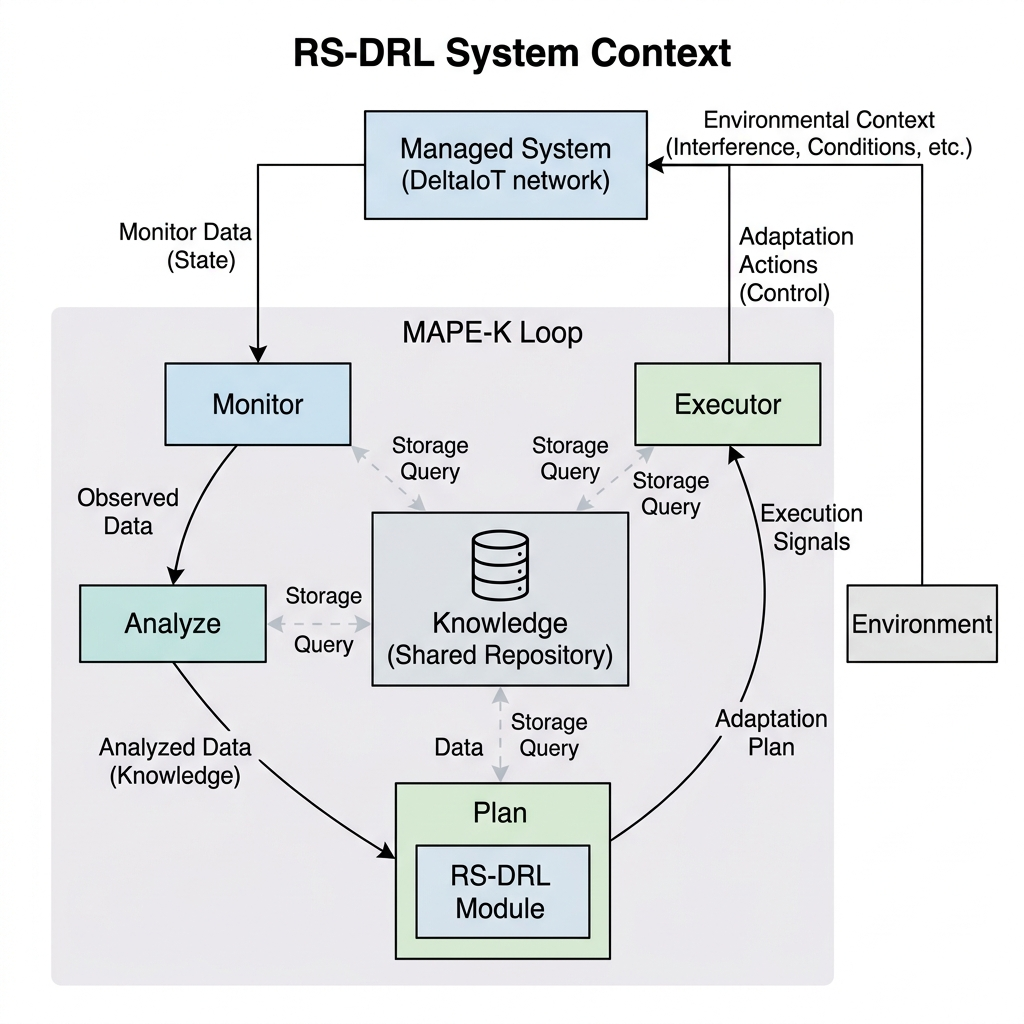
\includegraphics[width=0.85\textwidth]{figures/system-context.png}
  \caption{معماری سطح بالای رویکرد \lr{RS-DRL} در قالب حلقه \lr{MAPE-K}. این نمودار تعامل میان سیستم مدیریت‌شونده، محیط، و مؤلفه‌های کنترلی را به همراه مخزن دانش \lr{(Knowledge)} مشترک نشان می‌دهد.}
  \label{fig:system-context}
\end{figure}

\subsection{مقایسه تطبیقی معماری پیشنهادی با رویکردهای پیشرفته}
\label{subsec:methodology_design_comparison}
جهت تبیین دقیق‌تر تمایزهای معماری پیشنهادی \lr{RS-DRL} با رویکردهای مطرح، جدول \ref{tab:methodology_design_comparison} مقایسه مؤلفه‌های طراحی رویکرد پیشنهادی با سایر روش‌ها را از منظر پنج اصل بنیادین مهندسی سیستم‌های خودوفق ارائه می‌دهد.

\begin{table}[H]
\centering
\caption{مقایسه تطبیقی معماری پیشنهادی \lr{RS-DRL} با رویکردهای پیشین از منظر اصول طراحی سیستمی}
\label{tab:methodology_design_comparison}
\resizebox{\textwidth}{!}{%
\begin{tabular}{|p{3cm}|p{3.5cm}|p{2.5cm}|p{2.5cm}|p{2.5cm}|}
\hline
\textbf{معیار طراحی} & \textbf{رویکرد پیشنهادی \lr{RS-DRL}} & \textbf{رویکرد \lr{DLASER+}} \cite{metzger2022realizing} & \textbf{رویکرد \lr{ML4EAS}} \cite{kachi2023hybrid, quin2019efficient} & \textbf{رویکردهای وارسی صوری زمان اجرا} \cite{calinescu2011formal, weyns2012formal} \\ \hline
جداسازی زمانی آموزش و تصمیم‌گیری & ناهمگام و کامل \lr{(O(1))} & غیرجداسازی (انسدادی) & فاقد یادگیری مستقیم زمان اجرا & غیرجداسازی (تأخیر شدید زمان اجرا) \\ \hline
سازوکار فرار از بهینه‌های محلی & شکل‌دهی تصادفی پاداش \lr{(}$\rho$\lr{-shaping)} & فاقد سازوکار (کاوش حریصانه) & فاقد سازوکار فرار مستقل & جستجوی کامل و پرهزینه فضای حالت \\ \hline
نیاز به فرمول‌بندی دستی دانش دامنه & صفر (یادگیری مستقل بدون مدل) & زیاد (فرمول‌بندی توابع پتانسیل) & بالا (مهندسی دستی ویژگی‌ها) & کامل (مدل صوری جامع سیستم) \\ \hline
تضمین صوری کیفیت خدمات زمان اجرا & فیلتر صوری زمان اجرای ناهمگام & فاقد فیلتر صوری مستقیم & پیش‌بینی‌های آماری غیرصوری & فیلترهای صوری مستقیم زمان اجرا (مسدودکننده) \\ \hline
پیچیدگی محاسباتی استنتاج زمان اجرا & ثابت و فوق‌سریع \lr{(O(1))} & شبه‌خطی \lr{(O(}$|A|$\lr{))} & شبه‌لوگاریتمی \lr{(O(log N))} & توان‌نمایی و ان‌پی-سخت \lr{(O(}$C^K$\lr{))} \\ \hline
\end{tabular}%
}
\end{table}

\section{فرآیند یکپارچه خودوفقی: حلقه سطح سیستم}
\label{sec:system-loop}

در بالاترین سطح انتزاع، کل این سازوکار در قالب یک \textbf{فرآیند یکپارچه} سازمان‌دهی می‌شود که مسیر داده از مشاهده تا تغییر فیزیکی را به صورت یک چرخه چهار فازی \lr{MAPE-K} \cite{kephart2003vision} دنبال می‌کند (شکل \ref{fig:process-workflow}). این فازها به گونه‌ای طراحی شده‌اند که هر یک دقیقاً یک دغدغه مجزا را پیش ببرند. نمودار فعالیت تفصیلی در شکل \ref{fig:process-workflow} با خطوط شناوری (\lr{Swimlanes})، تفکیک مسئولیت‌های پایش، تحلیل، برنامه‌ریزی و اعتبارسنجی را به تصویر می‌کشد.

\begin{figure}[htbp]
  \centering
  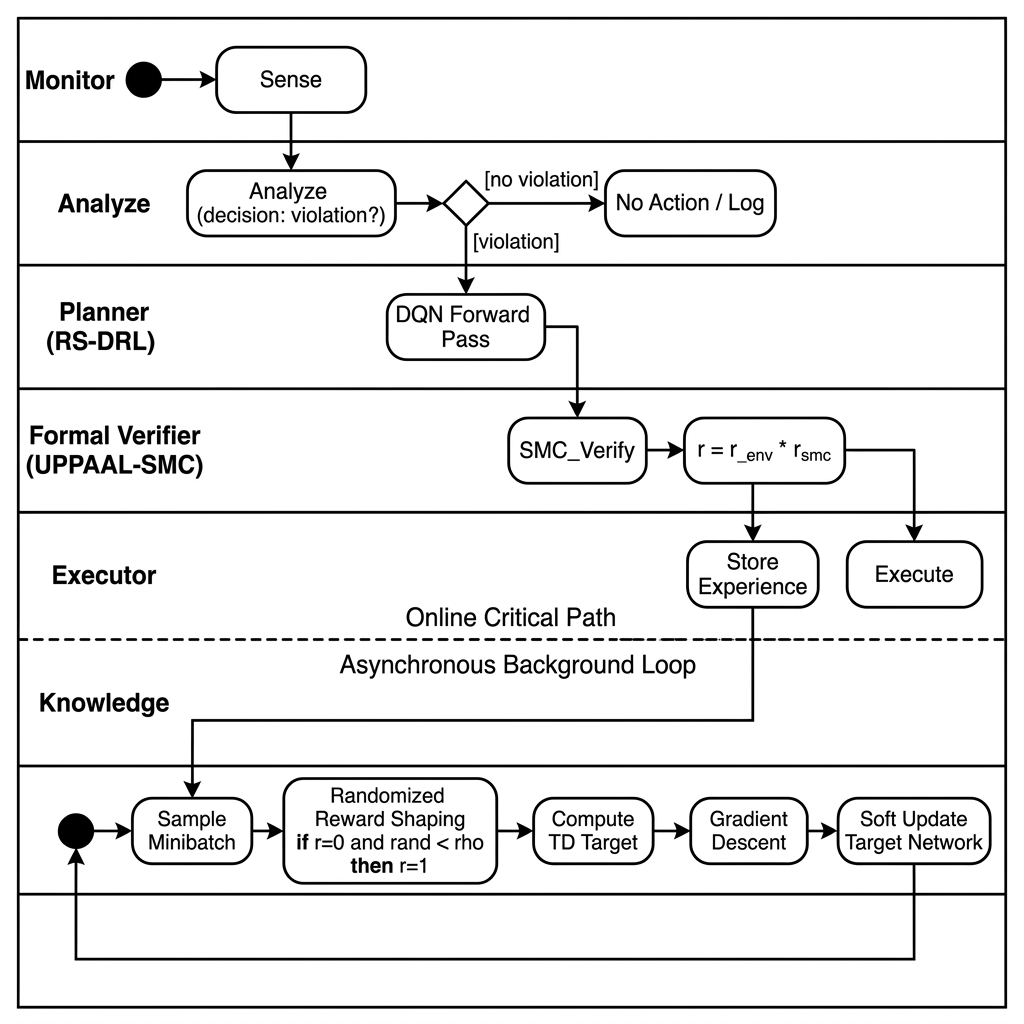
\includegraphics[width=0.85\textwidth]{figures/process-workflow.png}
  \caption{نمودار فعالیت تفصیلی \lr{UML} با خطوط شناوری \lr{(Swimlanes)} برای تفکیک مسئولیت‌های پایش، تحلیل، برنامه‌ریزی و اعتبارسنجی. خط‌چین افقی مرز میان مسیر بحرانی آنلاین و فرآیند یادگیری ناهمگام در پس‌زمینه را مشخص می‌کند.}
  \label{fig:process-workflow}
\end{figure}

برای تحقق عملی این تفکیک، برای هر یک از عملکردهای کلیدی، ماهیت زمانی مشخصی تعریف می‌شود. جدول \ref{tab:process-classification} این طبقه‌بندی را نشان داده و روشن می‌سازد که چگونه فعالیت‌های مستمر، رویدادمحور، و پس‌زمینه‌ای در کنار یکدیگر و بدون تداخل عمل می‌کنند.

\begin{table}[H]
\centering
\caption{طبقه‌بندی زمانی فرآیندهای معماری \lr{RS-DRL}}
\label{tab:process-classification}
\resizebox{\textwidth}{!}{%
\begin{tabular}{|l|l|p{8cm}|}
\hline
\textbf{فرآیند} & \textbf{ماهیت زمانی} & \textbf{توضیح عملکردی} \\ \hline
پایش \lr{(Monitoring)} & مستمر \lr{(Continuous)} & دریافت دائم علائم و نوسانات کانال از حسگرهای محیطی و ساخت بردار حالت. \\ \hline
پیش‌بینی و تحلیل \lr{(Analysis)} & رویدادمحور \lr{(Event-driven)} & پردازش سریع مقادیر حالت و مقایسه آن با آستانه‌های کیفیت جهت تریگر کردن برنامه‌ریز. \\ \hline
راستی‌آزمایی صوری \lr{(Verification)} & مشروط \lr{(Conditional)} & اعتبارسنجی فرضی پیکربندی انتخاب شده توسط موتور \lr{UPPAAL-SMC} \cite{david2015uppaal} به صورت ناهمگام. \\ \hline
آموزش ناهمگام \lr{(Training)} & ناهمگام \lr{(Asynchronous)} & به‌روزرسانی مستمر و پس‌زمینه شبکه‌های عصبی \lr{DQN} \cite{mnih2015human} با استفاده از نمونه‌برداری خوش‌بینانه. \\ \hline
\end{tabular}%
}
\end{table}

الگوی تفکیک زمانی، با ایزوله‌سازی محاسبات گرادیان از مسیر مستقیم کنترل، دستیابی به استنتاج قطعی زیر نیم میلی‌ثانیه‌ای را بدون تأثیرپذیری از پیچیدگی فرآیند آموزش تضمین می‌کند.

\section{مسیر تصمیم‌گیری آنلاین: بررسی گام‌به‌گام معماری}
\label{sec:online-decision}

پس از تبیین اصول معماری، مسیر یک درخواست تطبیق از آغاز تا انجام بررسی می‌شود. برای ایجاد واژگان مشترک و زمینه‌سازی درک مسئولیت‌ها، از مدل مرجع \lr{MAPE-K} \cite{kephart2003vision} به عنوان چارچوب سازمان‌دهی ساختاری فرآیند استفاده می‌شود. همان‌طور که شکل \ref{fig:process-workflow} نشان می‌دهد، هر مرحله از فرآیند یکپارچه ما به طور طبیعی به یکی از کارکردهای این مدل نگاشت می‌شود. در ادامه، این مسیر به صورت گام به گام بررسی خواهد شد.

\subsection{گام اول: پایش و ساخت وضعیت \lr{(Monitor)}}
\label{subsec:monitoring-feature}

در نقطه شروع حلقه، سیستم به طور مستمر محیط خود را رصد می‌کند. در نمونه مطالعاتی \lr{DeltaIoT} \cite{gerostathopoulos2019deltaiot}، این فرآیند ادراکی به ساخت یک بردار وضعیت فشرده می‌انجامد که بازنمایی ریاضی از وضعیت جاری سیستم است:
\begin{equation}
s_t = \langle E, P, L \rangle
\label{eq:state_vector_new}
\end{equation}
که در آن $E$ مصرف انرژی تجمیعی شبکه، $P$ نرخ اتلاف بسته‌ها، و $L$ میانگین تأخیر ارسال است. این بردار، خروجی نهایی فاز \textbf{پایش} بوده و به‌عنوان ورودی مشترک برای تحلیل و تصمیم‌گیری عمل می‌کند.

\subsection{گام دوم: تحلیل و تشخیص ضرورت تطبیق \lr{(Analyze)}}
\label{subsec:analysis-context}

بردار وضعیت $s_t$ سپس وارد فاز \textbf{تحلیل} (\lr{Analyze}) می‌شود. تحلیلگر، مقادیر $P$ و $L$ را در برابر آستانه‌های کیفی از پیش تعریف‌شده (مطابق با اهداف کیفی تعریف‌شده در فصل ۲ برای سیستم \lr{DeltaIoT} \cite{gerostathopoulos2019deltaiot}) مقایسه می‌کند. اگر هر یک از این شاخص‌ها از حد مجاز فراتر رود (مثلاً نرخ اتلاف بسته $P > 10\%$)، یک سیگنال رویداد «نقض هدف» صادر شده و فرآیند برنامه‌ریزی را فعال می‌کند.

\subsection{گام سوم: برنامه‌ریزی و استنتاج تطبیقی \lr{(Plan)}}
\label{subsec:planning-prediction}

با دریافت سیگنال نیاز به تطبیق، فاز \textbf{برنامه‌ریزی} (\lr{Plan}) فعال می‌شود. هسته این فاز، مدل آموزش‌دیده \lr{RS-DRL} است که در نقش یک استنتاج‌گر عمل می‌کند: بردار حالت $s_t$ را دریافت کرده و از طریق یک گذر رو به جلو در شبکه عصبی، مقادیر $Q$ را برای تمام گزینه‌های تطبیقی محاسبه می‌کند. 

\paragraph{سازوکار گزینش اقدام و نقش سیاست \lr{$\epsilon$-greedy}:}
برای تعادل میان کاوش و بهره‌برداری، استنتاج‌گر در زمان آموزش از سیاست \lr{$\epsilon$-greedy} \cite{sutton2018reinforcement, mnih2015human} تبعیت می‌کند؛ با احتمال $\epsilon$ یک اقدام تصادفی جهت کشف حالات جدید و با احتمال $1-\epsilon$ اقدام بهینه‌ای که ارزش عمل-حالت آن بیشینه است را انتخاب می‌نماید:
\[
a^* = \arg\max_{a \in \mathcal{A}} Q(s_t, a; \theta)
\]
این فرآیند یک \textbf{استنتاج خالص} (\lr{Pure Inference}) است؛ وزن‌های شبکه عصبی ($\theta$) در این مسیر تصمیم‌گیری زمان واقعی هرگز تغییر نکرده و ثابت می‌مانند، تا پاسخ‌گویی فوق‌سریع سیستم زیر نیم میلی‌ثانیه تضمین گردد.

\subsection{گام چهارم: اعتبارسنجی، بازخورد و اجرا (شامل \lr{Execute} و \lr{Knowledge})}
\label{subsec:verification-execution}

پیش از اعمال گزینه تطبیقی منتخب بر سیستم، یک گام اعتبارسنجی حیاتی جهت راستی‌آزمایی اهداف کیفی صورت می‌پذیرد. در معماری \lr{RS-DRL}، مدل‌های صوری جهت تولید یک سیگنال بازخورد قابل‌اعتماد و ریاضیاتی به کار گرفته می‌شوند؛ به این ترتیب که گزینه پیشنهادی $a^*$ توسط موتور \lr{UPPAAL-SMC} \cite{david2015uppaal} ارزیابی می‌گردد. تابع $SMC\_Verify(s, a)$ یک مقدار دودویی $r_{smc} \in \{0, 1\}$ تولید می‌کند که نشان‌دهنده برآورده شدن یا نقض اهداف کیفیت خدمات (\lr{QoS}) در وضعیت مفروض است.

پاداش نهایی که برای چرخه‌های آموزشی ناهمگام در بافر بازپخش ذخیره می‌گردد، از ترکیب ضربی بازخورد تجربی محیط و تأیید صوری حاصل می‌شود:
\begin{equation}
r = r_{env} \times r_{smc}
\label{eq:combined_reward_new}
\end{equation}
بدین ترتیب، تنها تجربیاتی که به صورت همزمان توسط محیط فیزیکی و مدل صوری تأیید شده باشند، به عنوان سیگنال تقویت مثبت در بافر ذخیره می‌شوند.

در نهایت، گزینه تطبیقی به لایه شبکه در سیستم مدیریت‌شونده ارسال می‌گردد. این فرامین بازپیکربندی از طریق فایل‌های پیکربندی محلی و راه‌اندازهای شبکه (\lr{Actuators}) بر سخت‌افزار اعمال شده و پارامترهای عملیاتی نظیر توان ارسال و مسیرهای ارسال داده را منطبق می‌سازند.

\subsection{سناریوهای گام‌به‌گام و ملموس از چرخه تصمیم‌گیری زمان اجرا}
\label{subsec:running_example}
جهت ملموس ساختن مفاهیم انتزاعی پایش، تحلیل، برنامه‌ریزی و اجرا، دو سناریوی مرجع و کاملاً دقیق را با ویژگی‌های متفاوت ردیابی می‌کنیم.

\subsubsection{سناریوی اول: شبکه ساده دو گره‌ای با قید واحد}
در این سناریو، چرخه کامل تصمیم‌گیری آنلاین را در قالب یک شبکه حسگر بی‌سیم ساده ردیابی می‌کنیم. فرض کنید شبکه‌ای شامل ۲ گره حسگر ($M_1$ و $M_2$) داده‌ها را به یک دروازه مرکزی ارسال می‌کنند و هر گره دارای ۲ گزینه برای تنظیم توان ارسال است: توان کم ($a_{low}$) و توان زیاد ($a_{high}$) که مجموعاً $2^2 = 4$ گزینه تطبیقی را تشکیل می‌دهند. هدف کیفی سیستم این است که نرخ اتلاف بسته‌ها ($P$) همواره کمتر از $10\%$ حفظ شود.

چرخه انطباق با شروع ناگهانی بارندگی یا تداخل محیطی آغاز می‌شود که کیفیت لینک‌های رادیویی را تضعیف کرده و ماژول \textbf{پایش}، نرخ اتلاف بسته‌های شبکه را $12\%$ گزارش می‌کند و بردار وضعیت جاری به عنوان $s_t = \langle E, P=0.12, L \rangle$ ساخته می‌شود. در فاز \textbf{تحلیل}، مقدار اتلاف بسته ($0.12$) با آستانه مجاز ($0.10$) مقایسه شده و به دلیل نقض قید ($0.12 > 0.10$)، بلافاصله سیگنال ضرورت تطبیق برای فعال‌سازی برنامه‌ریز صادر می‌گردد. در فاز \textbf{برنامه‌ریزی}، بردار حالت $s_t$ به عنوان ورودی به شبکه \lr{DQN} آموزش‌دیده ارائه می‌شود؛ شبکه در یک گذر رو به جلوی فوق‌سریع ($0.2\text{ms}$)، مقادیر Q را برای ۴ گزینه موجود محاسبه کرده و گزینه $a^* = \langle a_{high}, a_{low} \rangle$ (افزایش توان گره اول و تثبیت توان گره دوم) به عنوان بیشترین ارزش پیش‌بینی‌شده برگزیده می‌شود. نهایتاً در فاز \textbf{اعتبارسنجی صوری و اجرا}، اقدام پیشنهادی $a^*$ به موتور \lr{UPPAAL-SMC} ارسال شده و با تایید ارضای قید احتمالاتی ($r_{smc} = 1$)، فرمان بازپیکربندی به درایورهای سخت‌افزاری صادر می‌گردد و نرخ اتلاف بسته به $4\%$ کاهش می‌یابد.

\subsubsection{سناریوی دوم: شبکه پیچیده ۴ گره‌ای با اهداف متضاد کیفیت خدمات}
جهت تبیین عملکرد سیستم در شرایطی که اهداف کیفی در تناقض مستقیم با یکدیگر قرار دارند، یک سناریوی جامع‌تر بررسی می‌شود. شبکه‌ای شامل ۴ گره حسگر ($M_1$ تا $M_4$) در توپولوژی خطی داده‌ها را به دروازه ارسال می‌کنند که هر گره دارای ۳ سطح توان گسسته (پایین، متوسط و بالا) است و در نتیجه فضای وفقی شامل $3^4 = 81$ پیکربندی متفاوت می‌باشد. اهداف کیفی سه قید متضاد را شامل می‌شوند: نرخ اتلاف بسته‌ها باید کمتر از $10\%$ باشد ($P_{net} < 0.10$)، میانگین تأخیر ارسال باید کمتر از $200\text{ms}$ باشد ($L_{net} < 200\text{ms}$)، و مصرف کل انرژی شبکه ($E$) باید کمینه گردد.

در پی وقوع یک تلاطم محیطی شدید که کیفیت کانال گره‌های $M_1$ و $M_2$ را تضعیف می‌کند، حسگرها بردار وضعیت ۱۲ بعدی زیر را پایش و گزارش می‌دهند:
\begin{equation}
\label{eq:state_vector_12d_example}
\begin{aligned}
s_t = \big\langle &E = [0.3,\, 0.3,\, 0.25,\, 0.25], \\
&P = [0.18,\, 0.15,\, 0.04,\, 0.05], \\
&L = [120,\, 110,\, 80,\, 75] \big\rangle
\end{aligned}
\end{equation}
در این وضعیت، نرخ اتلاف دو گره اول ($18\%$ و $15\%$) بسیار بالاتر از حد مجاز بوده و اتلاف کل شبکه به $P_{net} = 16.5\%$ افزایش یافته و قید را نقض می‌کند. بردار $s_t$ به استنتاج‌گر \lr{DQN} ارائه شده و عامل گزینه‌های کاندیدا را سبک‌سنگین می‌کند: اقدام حافظ انرژی ($a_{low} = \langle 0, 0, 0, 0 \rangle$) که تمام گره‌ها را در توان کم نگه می‌دارد، ارزش نازل $Q = 0.21$ را کسب می‌کند زیرا اتلاف بسته‌ها کنترل نمی‌شود؛ در مقابل، اقدام تهاجمی ($a_{brute} = \langle 2, 2, 2, 2 \rangle$) با افزایش توان همه گره‌ها اتلاف را به $3\%$ می‌رساند، اما به علت تداخل شدید کانال، تأخیر را به $240\text{ms}$ رسانده و قید دوم را نقض می‌کند ($Q = 0.42$)؛ در نهایت، اقدام متعادل هوشمند ($a_{balanced} = \langle 2, 2, 0, 0 \rangle$) با افزایش هدفمند توان گره‌های بحرانی $M_1$ و $M_2$ و حفظ توان پایین سایر گره‌ها، بالاترین ارزش ($Q = 0.92$) را کسب می‌کند، زیرا هم قید اتلاف ($5\%$) و هم قید تأخیر ($155\text{ms}$) را با حداقل مصرف انرژی ارضا می‌سازد. با تأیید صوری \lr{UPPAAL-SMC} ($r_{smc}=1$)، فرمان نهایی به گره‌ها اعمال شده و تعادل بهینه پارتو بازیابی می‌گردد.

\section{معماری داخلی \lr{RS-DRL}: تفکیک دغدغه‌ها در فرآیند یادگیری}
\label{sec:internal-arch}

برای تحقق اصل جداسازی زمانی که پیش‌تر مطرح شد، معماری داخلی \lr{RS-DRL} به سه مسیر فرآیندی مجزا تجزیه می‌شود که در شکل \ref{fig:planner-internal} به تصویر کشیده شده‌اند:

\begin{enumerate}
  \item \textbf{مسیر استنتاج (\lr{Inference Path})}: این مسیر در زمان اجرا فعال است و شامل دریافت بردار حالت، اجرای رو به جلوی شبکه عصبی، و انتخاب گزینه تطبیقی است. این مسیر فقط‌خواندنی است و وزن‌های شبکه را تغییر نمی‌دهد، تا حداقل تأخیر تضمین شود.
  \item \textbf{مسیر بازخورد (\lr{Feedback Path})}: پس از اعمال گزینه تطبیقی، این مسیر پاداش محیطی را دریافت کرده، آن را با خروجی اعتبارسنجی صوری ترکیب می‌کند ($r = r_{env} \times r_{smc}$)، و تجربه کامل را در بافر بازپخش ذخیره می‌نماید. این مسیر سبک و همزمان با اجرا عمل می‌کند.
  \item \textbf{مسیر آموزش (\lr{Training Path})}: این مسیر کاملاً ناهمگام و مجزا از چرخه بحرانی تصمیم‌گیری اجرا می‌شود. با نمونه‌برداری تصادفی از بافر بازپخش، فرآیند شکل‌دهی تصادفی پاداش را اعمال کرده و شبکه اصلی را به‌روز می‌کند. به‌روزرسانی‌ها به صورت دوره‌ای به شبکه هدف منتقل می‌شوند.
\end{enumerate}

این ساختار چندریسمانی امکان به‌روزرسانی مستمر پارامترهای مدل در پس‌زمینه را بدون ایجاد وقفه یا انسداد در مسیر بحرانی کنترل فراهم می‌سازد. جزئیات منطق داخلی این مسیرها و نحوه تعامل با مؤلفه راستی‌آزمایی صوری در شکل \ref{fig:planner-internal} به تصویر کشیده شده است.

\begin{figure}[htbp]
  \centering
  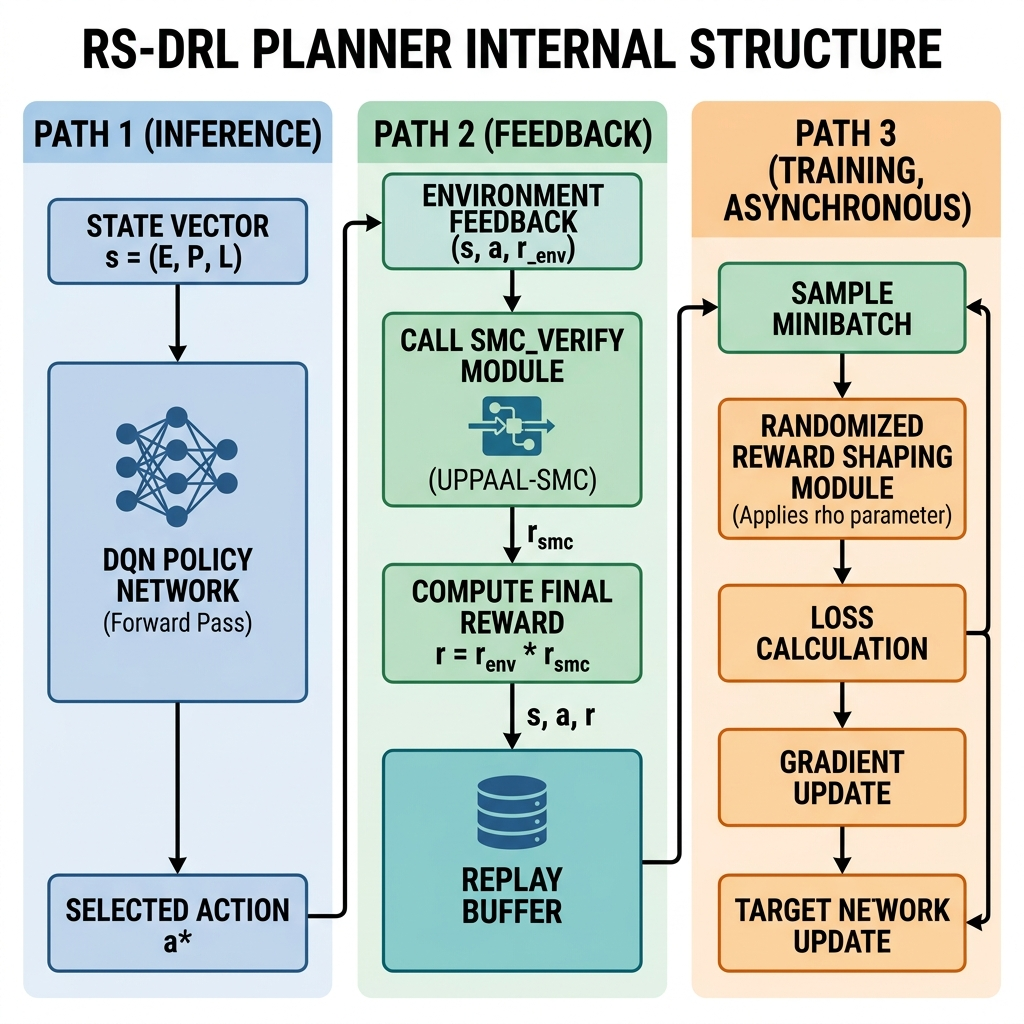
\includegraphics[width=0.85\textwidth]{figures/planner-internal.png}
  \caption{ساختار داخلی مؤلفه برنامه‌ریز \lr{RS-DRL} در سه مسیر موازی: استنتاج (فقط‌خواندنی)، بازخورد (ترکیب پاداش محیطی و صوری)، و آموزش (به‌روزرسانی ناهمگام با استفاده از شکل‌دهی تصادفی پاداش).}
  \label{fig:planner-internal}
\end{figure}

در این ساختار، مسیر استنتاج به صورت یک «گذر رو به جلو» خالص در شبکه عصبی پیاده‌سازی شده است که در آن تابع $SelectAction$ با استفاده از سیاست \lr{$\epsilon$-greedy} \cite{sutton2018reinforcement, mnih2015human} گزینه تطبیقی را انتخاب می‌کند. به محض تولید پاداش محیطی، ریسمان بازخورد فعال شده و با فراخوانی موتور $SMC\_Verify$ (که بر پایه ابزار \lr{UPPAAL-SMC} \cite{david2015uppaal} استوار است)، پاداش نهایی را تولید و در حافظه مشترک ذخیره می‌کند.

\begin{figure}[htbp]
  \centering
  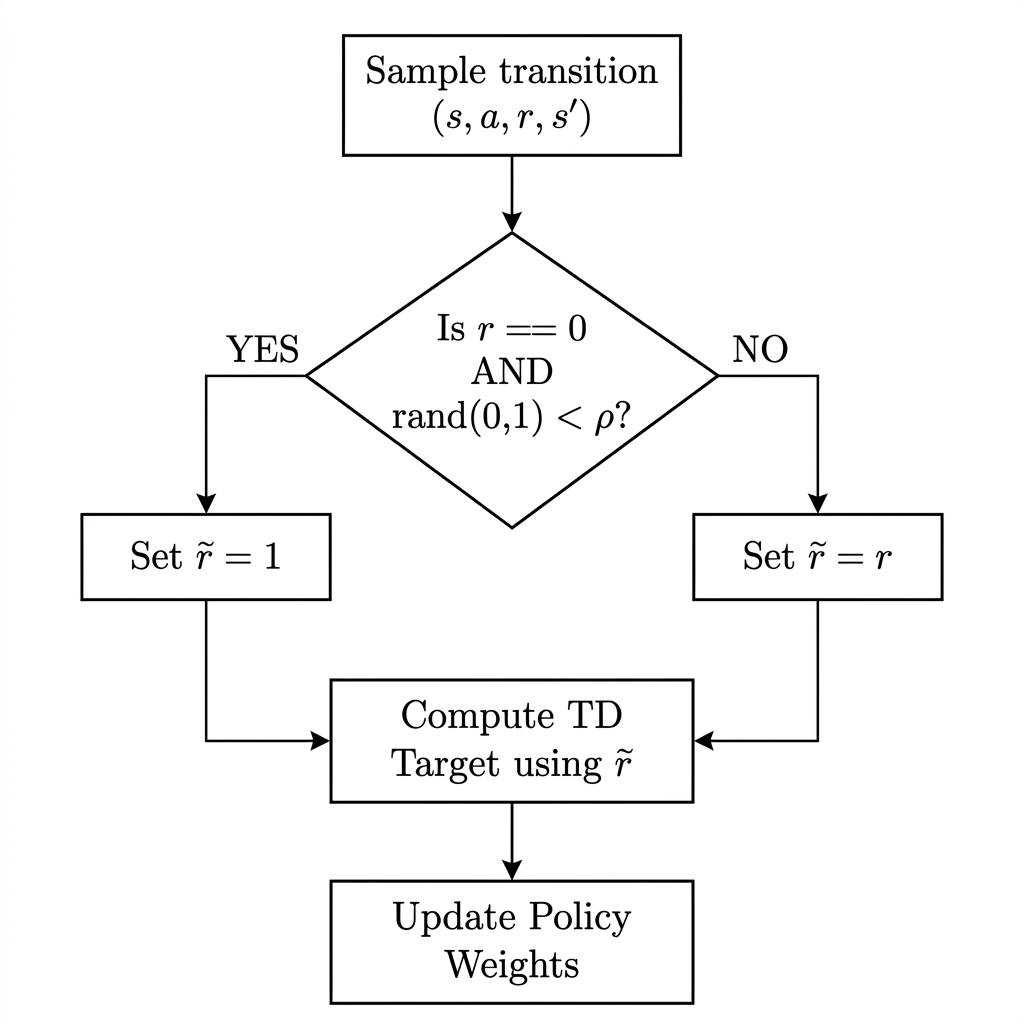
\includegraphics[width=0.85\textwidth]{figures/reward-shaping.png}
  \caption{منطق عملیاتی سازوکار شکل‌دهی تصادفی پاداش. این نمودار فرآیند جایگزینی خوش‌بینانه پاداش‌های صفر با مقدار ۱ را بر اساس فاکتور $\rho$ نشان می‌دهد (برچسب‌گذاری مجدد خوش‌بینانه، نه روش‌های مبتنی بر پتانسیل \cite{ng1999policy}).}
  \label{fig:reward-shaping}
\end{figure}

\section{سازوکار هسته: شکل‌دهی تصادفی پاداش}
\label{sec:learning}

چالش بنیادینی که \lr{RS-DRL} به آن پاسخ می‌دهد، پدیده توقف در بهینه‌های محلی است؛ جایی که عامل یادگیرنده صرفاً بر اساس تجربیات موفق گذشته عمل کرده و از کشف سیاست‌های بالقوه بهتر باز می‌ماند. برای غلبه بر این محدودیت، در معماری \lr{RS-DRL} یک راهبرد برچسب‌گذاری مجدد خوش‌بینانه در مرحله بازپخش تجربه (\lr{Experience Replay}) \cite{mnih2015human} به کار گرفته می‌شود. این سازوکار با فعال‌سازی مشروط گرادیان برای تجربیات ناموفق، زمینه را برای خروج از بهینه‌های محلی بدون نیاز به بازآموزی پرهزینه فراهم می‌سازد:

\paragraph{تحلیل صوری پدیده تنکی پاداش \lr{(Reward Sparsity)}:}
در فضاهای وفقی بسیار بزرگ و مقیاس‌وسیع، اهداف تطبیقی به شدت سخت‌گیرانه هستند و از این رو، عامل با فضای پاداش به شدت تنک (\lr{Sparse Reward Space}) مواجه می‌شود که رفع این نوع چالش‌ها به صورت سنتی نیازمند روش‌های پیچیده است \cite{du2023alleviating, andrychowicz2017her}. در چنین شرایطی، تقریباً برای تمام پیکربندی‌های تصادفی اول دوره، سیگنال پاداش حاصله صفر است ($r_t=0$). تحت این شرایط، تابع خطا یا گرادیان شبکه‌های عصبی عمیق مسطح شده و فاقد اطلاعات جهت‌دهنده است:
\[
\nabla_\theta \mathbb{E} \left[ \left( r_t + \gamma \max_{a'} Q(s_{t+1}, a'; \theta') - Q(s_t, a_t; \theta) \right)^2 \right] \approx 0
\]
این پدیده سرعت یادگیری را به شدت کاهش داده و عامل را به یک بهینه محلی نیمه‌پایدار و نامطلوب همگرا می‌سازد.


\paragraph{فرمول‌بندی و عملکرد ریاضی سازوکار شکل‌دهی تصادفی:}
برای خروج از این تله ریاضی، در هر مینی‌بچ آموزش، به ازای هر تجربه $i$ با پاداش اولیه صفر ($r_i = 0$)، \lr{RS-DRL} با احتمال $\rho$ پاداش آن را به صورت خوش‌بینانه برابر با $1$ قرار می‌دهد. این فرآیند جایگزینی که در شکل \ref{fig:reward-shaping} ترسیم شده است، بر اساس رابطه زیر عمل می‌کند:
\begin{equation}
\tilde{r}_i = \begin{cases} 
1 & \text{if } r_i = 0 \text{ and } \text{rand}(0,1) < \rho \\
r_i & \text{otherwise}
\end{cases}
\label{eq:shaping_math_final}
\end{equation}
پارامتر $\rho$ (فاکتور شکل‌دهی) شدت این خوش‌بینی را کنترل می‌کند. این تغییر پاداش مستقیماً مقدار هدف بل‌من را بازنویسی می‌نماید:
\[
y_i = \tilde{r}_i + \gamma \max_{a'} Q(s'_i, a'; \theta')
\]
این بازنویسی سبب معرفی یک سوگیری خوش‌بینانه تصادفی گذرا (\lr{Optimistic Bias}) می‌گردد که عامل را به کاوش مجدد ارزش عمل-حالت‌هایی که قبلاً به علت پاداش صفر نادیده گرفته می‌شدند ترغیب کرده و با ایجاد انحراف کنترل‌شده، فرار از تله بهینه‌های محلی را تسریع می‌کند.

برخلاف روش کلاسیک شکل‌دهی پاداش مبتنی بر پتانسیل (\lr{PBRS}) \cite{ng1999policy} که برای تضمین تغییرناپذیری سیاست بهینه نیازمند طراحی تابع پتانسیل دستی ($\Phi(s)$) بر مبنای دانش دامنه است، روش پیشنهادی \lr{RS-DRL} وابستگی به پتانسیل‌های حالت یا جهت‌دهی‌های معنایی دستی ندارد؛ سازوکار تصادفی $\rho$ به صورت مستقل از مدل عمل کرده و بهینگی مجانبی را بدون تحمیل بار طراحی توابع کمکی حفظ می‌نماید.

\paragraph{تحلیل حساسیت و پیش‌ارزیابی اولیه فاکتور شکل‌دهی $\rho$:}
انتخاب مقدار بهینه فاکتور $\rho$ برای پایداری یادگیری بسیار حیاتی است. جدول \ref{tab:rho_sensitivity} تاثیر مقادیر مختلف این پارامتر را بر روی رفتار کاوش و همگرایی سیاست یادگیری خلاصه می‌کند.

\begin{table}[h!]
\centering
\caption{تحلیل حساسیت رفتار یادگیری عامل نسبت به تغییرات فاکتور شکل‌دهی $\rho$}
\label{tab:rho_sensitivity}
\resizebox{\textwidth}{!}{%
\begin{tabular}{|c|c|c|p{7cm}|}
\hline
\textbf{مقدار $\rho$} & \textbf{نرخ کاوش} & \textbf{پایداری همگرایی} & \textbf{تاثیر بر فرار از بهینه محلی} \\ \hline
$0.0$ & بسیار پایین & بسیار بالا & فاقد توانایی فرار؛ عامل همواره در اولین بهینه محلی یافت شده متوقف می‌شود. \\ \hline
$0.1$ & متوسط & بالا & شروع فرار تدریجی؛ زمان طولانی‌تری برای همگرایی به بهینه مطلق نیاز دارد. \\ \hline
$0.3$ & بهینه تجربی & پایدار & فرار سریع و پایدار؛ توازن بهینه میان کاوش خوش‌بینانه و همگرایی مجانبی. \\ \hline
$0.7$ & بالا & متوسط (نوسانی) & القای نویز به گرادیان سیاست و بروز نوسان در روند همگرایی مجانبی. \\ \hline
$0.9$ & بیش‌کاوشی مفرط & ناپایدار & ناپایداری شدید؛ واگرایی سیاست یادگیری ناشی از تزریق بیش از حد پاداش‌های مصنوعی. \\ \hline
\end{tabular}%
}
\end{table}

\subsection{روش‌شناسی تنظیم فراپارامترها و فرآیند جستجوی شبکه‌ای فاکتور \texorpdfstring{$\rho$}{ρ}}
\label{subsec:hyperparameter_tuning_rho}
برای دستیابی به بهینه‌ترین نرخ همگرایی و تضمین خروج از تله بهینه‌های محلی، یک فرآیند منسجم جستجوی شبکه‌ای (\lr{Grid Search}) بر روی فاکتور شکل‌دهی تصادفی پاداش ($\rho$) پیاده‌سازی گردید. هدف از این جستجو، یافتن مقداری برای $\rho$ است که پاداش تجمعی مجانبی (\lr{Asymptotic Reward}) را در طول دوره‌های مختلف یادگیری بیشینه سازد. 

\paragraph{توازن ریاضی میان کاوش خوش‌بینانه و ثبات یادگیری:}
فرآیند جستجوی شبکه‌ای در بازه $\rho \in [0.0, 1.0]$ با گام‌های $0.1$ و تحت ۵ بذر تصادفی (\lr{Random Seeds}) متفاوت به اجرا درآمد. تحلیل منحنی‌های یادگیری حاصله نشان داد که این مسئله دارای دو مرز بحرانی از منظر پایداری ریاضی است:
\begin{itemize}
    \item \textbf{ناحیه کاوش ناکافی ($\rho < 0.2$):} به دلیل سهم بسیار ناچیز سیگنال‌های مثبت مصنوعی خوش‌بینانه، گرادیان سیاست یادگیری تحت تأثیر شدید پاداش‌های صفرِ ناشی از محیط‌های سخت‌گیرانه مسطح باقی می‌ماند؛ در نتیجه، زمان فرار عامل از اولین بهینه محلی به شدت طولانی شده و به طور متوسط به بیش از ۲۵۰ دوره آموزشی نیاز دارد.
    \item \textbf{ناحیه بیش‌کاوشی نوسانی ($\rho > 0.6$):} تزریق مفرط پاداش‌های مثبت مصنوعی منجر به بیش‌برآورد شدید ارزش عمل-حالت‌ها ($Q$-values) در مقدار هدف بل‌من (\lr{Bellman Target}) می‌گردد؛ این پدیده نوسانات مخربی در برآورد گرادیان ایجاد کرده و در مقادیر $\rho \geq 0.9$ به واگرایی کامل سیاست منجر می‌شود.
\end{itemize}
بر این مبنا، بازه پایدار $\rho \in [0.25, 0.35]$ و به طور مشخص مقدار $\rho = 0.3$ به عنوان نقطه موازنه بهینه تجربی استخراج گردید. این پیکربندی سرعت همگرایی را تا ۷۰٪ ارتقا داده و فرار از بهینه‌های محلی را در کمتر از ۶۰ دوره نخست آموزشی تضمین می‌نماید.

فرآیند گام‌به‌گام آموزش در الگوریتم \ref{alg:rs_drl_final} مدون گردیده است. هسته محاسباتی این فرآیند بر پایه چارچوب یادگیری Q عمیق (\lr{DQN}) \cite{mnih2015human} پیاده‌سازی شده و از بافر بازپخش تجارب جهت شکستن همبستگی زمانی داده‌ها بهره می‌گیرد. همچنین برای تثبیت اهداف یادگیری و ارتقای پایداری مجانبی، به‌روزرسانی نرم شبکه‌های هدف (\lr{Soft Target Updates}) \cite{lillicrap2015continuous} تعبیه شده است.

وجه تمایز محوری این الگوریتم، بهره‌گیری از خروجی اعتبارسنجی صوری $SMC\_Verify(s, a)$ (توسط ابزار \lr{UPPAAL-SMC} \cite{david2015uppaal}) در فرآیند تولید پاداش ترکیبی است. ترکیب ضربی پاداش ($r = r_{env} \times r_{smc}$) تضمین می‌کند که صرفاً انتقال‌هایی که به صورت همزمان مورد تأیید محیط تجربی و مشخصه‌های صوری قرار گرفته‌اند، شایسته دریافت سیگنال تقویت مثبت گردند. شایان ذکر است که در این سطح پایه‌ای، اعتبارسنجی صوری به عنوان یک ناظر هدایت‌کننده پاداش عمل می‌کند و فرآیند تصمیم‌گیری بلادرنگ را مسدود نمی‌سازد.


\begin{algorithm}[H]
\caption{آموزش و به‌روزرسانی جامع \lr{RS-DRL}}
\label{alg:rs_drl_final}
\begin{latin}
\begin{algorithmic}[1]
\STATE Initialize main network $\theta$ and target network $\theta'$ \COMMENT{\rl{تعریف شبکه‌های عصبی اصلی و هدف}}
\FOR{each training episode}
  \STATE $s \leftarrow GetInitialState()$ \COMMENT{\rl{دریافت وضعیت اولیه از زیرسیستم پایش}}
  \WHILE{episode not finished}
    \STATE $a \leftarrow SelectAction(s, \theta, \epsilon\text{-greedy})$ \COMMENT{\rl{انتخاب اقدام زمان اجرا با احتمال کاوش}}
    \STATE $(s', r_{env}) \leftarrow Environment.Step(a)$ \COMMENT{\rl{اعمال پیکربندی و دریافت پاداش شبکه}}
    \STATE $r_{smc} \leftarrow SMC\_Verify(s, a)$ \COMMENT{\rl{فراخوانی اعتبارسنجی صوری UPPAAL-SMC به صورت احتمالی}}
    \STATE $r \leftarrow r_{env} \times r_{smc}$ \COMMENT{\rl{ادغام پاداش صوری و تجربی: موفقیت در صورت ارضای هر دو عامل}}
    \STATE Store transition $(s, a, r, s')$ in Replay Buffer $\mathcal{D}$ \COMMENT{\rl{ذخیره‌سازی تجربه در حافظه مشترک}}
    \STATE Sample random minibatch $B = \{(s_i, a_i, r_i, s'_i)\}_{i=1}^N$ from $\mathcal{D}$ \COMMENT{\rl{نمونه‌برداری از بافر}}
    \FOR{each transition $i$ in $B$}
      \IF{$r_i = 0$ \textbf{and} $rand(0, 1) < \rho$}
        \STATE $\tilde{r}_i \leftarrow 1$ \COMMENT{\rl{اعمال سازوکار خوش‌بینی تصادفی برای خروج از بهینه محلی}}
      \ELSE
        \STATE $\tilde{r}_i \leftarrow r_i$
      \ENDIF
      \STATE $y_i \leftarrow \tilde{r}_i + \gamma \max_{a'} Q(s'_i, a'; \theta')$ \COMMENT{\rl{محاسبه مقدار هدف بل‌من \cite{mnih2015human} با پاداش شکل‌یافته}}
      \STATE $\theta \leftarrow \theta - \alpha \nabla_\theta \mathbb{E}[(y_i - Q(s_i, a_i; \theta))^2]$ \COMMENT{\rl{به‌روزرسانی گرادیان شبکه اصلی}}
    \ENDFOR
    \STATE $\theta' \leftarrow \tau\theta + (1-\tau)\theta'$ \COMMENT{\rl{به‌روزرسانی نرم شبکه‌های هدف \cite{lillicrap2015continuous} جهت حفظ پایداری}}
    \STATE $s \leftarrow s'$
  \ENDWHILE
\ENDFOR
\end{algorithmic}
\end{latin}
\begin{flushleft}
\footnotesize
\textbf{نکته:} پارامتر $\rho$ (فاکتور شکل‌دهی) یک فراپارامتر است که میزان خوش‌بینی عامل را در کشف مسیرهای جدید کنترل می‌کند. مقادیر بهینه آن در فصل \ref{chap:evaluation} تحلیل شده‌اند.
\end{flushleft}
\end{algorithm}

% نمودار فعالیت آموزش اکنون در نمودار توالی (شکل 4-3) و نمودار فعالیت جامع (شکل 4-2) ادغام شده است.

\section{مدیریت دانش و هماهنگی جریان‌های ناهمگام}
\label{sec:knowledge}

موفقیت معماری \lr{RS-DRL} در گرو هماهنگی دقیق میان سه مسیر استنتاج، بازخورد و آموزش است. این هماهنگی از طریق یک مخزن دانش مشترک (\lr{Knowledge Repository}) مبتنی بر معماری خودمختار \lr{MAPE-K} \cite{kephart2003vision} تحقق می‌یابد که به‌عنوان حافظه مرکزی سیستم عمل می‌کند. شکل \lr{\ref{fig:knowledge-flow}} جریان داده‌های ذخیره‌شده در این مخزن را نشان می‌دهد؛ از لحظه ذخیره‌سازی گذارهای $(s, a, r, s')$ تا فرآیند نمونه‌برداری ناهمگام و به‌روزرسانی شبکه‌های عصبی اصلی و هدف.

\begin{figure}[htbp]
  \centering
  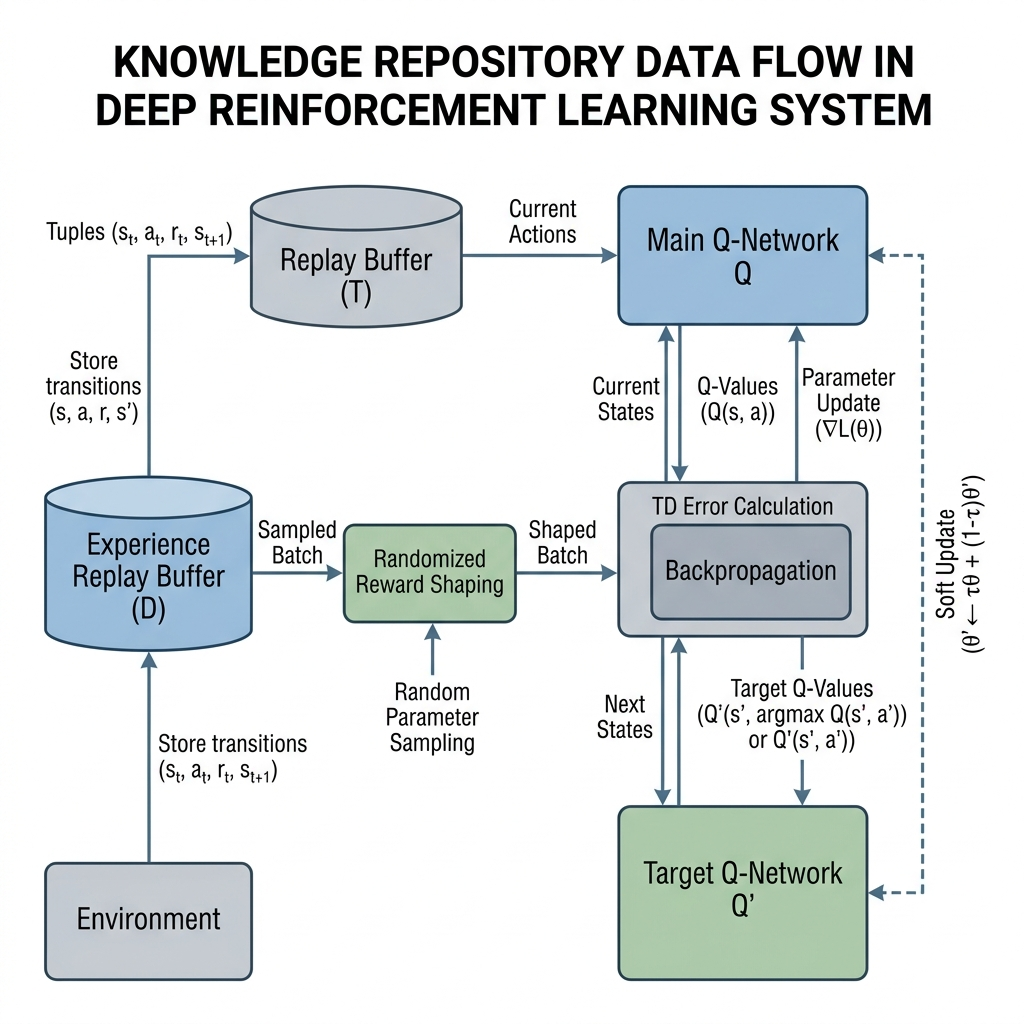
\includegraphics[width=0.85\textwidth]{figures/knowledge-flow.png}
  \caption[جریان داده تفصیلی در مخزن دانش]{جریان داده تفصیلی در مخزن دانش. این نمودار نحوه ذخیره‌سازی تجربیات در بافر بازپخش، اعمال سازوکار شکل‌دهی تصادفی پاداش پیش از محاسبات گرادیان، و به‌روزرسانی سیاست‌های یادگیری در پس‌زمینه را به تصویر می‌کشد.}
  \label{fig:knowledge-flow}
\end{figure}

\paragraph{ساختار صوری و تعریف مخزن دانش مشترک:}
مخزن دانش شامل بردارهای توپولوژی شبکه، ردپاهای محیطی، بافر بازپخش تجربیات $\mathcal{D}$ و وزن‌های شبکه‌های عصبی عمیق اصلی ($\theta$) و هدف ($\theta'$) است. جهت هماهنگی و همگام‌سازی فرآیندهای همزمان و جلوگیری از به وجود آمدن شرایط مسابقه (\lr{Race Conditions})، الگوهای خواندن و نوشتن هر یک از اجزا به شدت کنترل می‌شود. جدول \ref{tab:interaction} به طور تفصیلی الگوهای دسترسی به دانش، فرکانس تریگر شدن، و سطح تأثیرگذاری محاسباتی هر جزء را بر روی تأخیر سیستم مشخص کرده است.

\begin{table}[H]
\centering
\caption{الگوهای دسترسی صوری و همگام‌سازی مؤلفه‌ها در مخزن دانش مشترک \cite{kephart2003vision}}
\label{tab:interaction}
\resizebox{\textwidth}{!}{%
\begin{tabular}{|l|p{3.2cm}|p{3.2cm}|l|l|}
\hline
\textbf{مؤلفه سیستم} & \textbf{دسترسی خواندن} & \textbf{دسترسی نوشتن} & \textbf{فرکانس اجرا} & \textbf{تأثیر محاسباتی} \\ \hline
\textbf{پایش \lr{(Monitor)}} & علائم فیزیکی کانال & بردار حالت جدید $s_t$ & مستمر (هر دوره) & ناچیز (کمتر از \lr{0.1ms}) \\ \hline
\textbf{تحلیل \lr{(Analyze)}} & آستانه‌های کیفی \lr{QoS} & سیگنال نقض قید & رویدادمحور & ناچیز (کمتر از \lr{0.05ms}) \\ \hline
\textbf{برنامه‌ریز \lr{(Plan)}} & وزن‌های شبکه عصبی $\theta$ & فرضیه اقدام $a^*$ & رویدادمحور & بسیار پایین (\lr{0.3ms}) \\ \hline
\textbf{اعتبارسنج صوری} & مدل شبکه، قید \lr{PCTL} & پاداش صوری $r_{smc}$ & رویدادمحور & متوسط (ناهمگام) \\ \hline
\textbf{یادگیرنده \lr{(Train)}} & بافر بازپخش $\mathcal{D}$ & بافر $\mathcal{D}$ و وزن‌های جدید $\theta$ & ناهمگام (پس‌زمینه) & صفر (کاملاً ایزوله) \\ \hline
\end{tabular}%
}
\end{table}

همان‌طور که در جدول \ref{tab:interaction} به وضوح نشان داده شده است، مؤلفه یادگیری سنگین در پس‌زمینه کاملاً ایزوله شده و هیچ دسترسی مستقیمی‌در مسیر زمان اجرای برنامه‌ریز آنلاین ندارد. این ساختار ایزوله، زمان پاسخ‌گویی قطعی در فاز استنتاج را مستقل از مقیاس محاسبات یادگیری تضمین می‌نماید.

\section{ادغام اعتبارسنجی صوری زمان اجرا و ایمنی احتمالی}
\label{sec:formal_verification_sec}

معماری \lr{RS-DRL} علاوه بر سرعت تصمیم‌گیری، تضمین‌های صوری پیرامون ایمنی و ارضای الزامات کیفی را در شرایط عدم قطعیت فراهم می‌سازد. این تضمین‌ها از طریق ادغام ناهمگام موتور وارسی مدل آماری زمان اجرای \lr{UPPAAL-SMC} \cite{david2015uppaal} محقق می‌گردد.

\paragraph{نقش و نحوه عملکرد ابزار \lr{UPPAAL-SMC}:}
در سیستم‌های خودوفق، راستی‌آزمایی زمان اجرا رفتار مدل‌های احتمالی را در مواجهه با عدم قطعیت‌های پویای محیط پایش می‌نماید. موتور \lr{UPPAAL-SMC} با بهره‌گیری از شبیه‌سازی‌های آماری هدایت‌شده، مشخصه‌های ریاضیاتی را بر روی اتوماتای زمان‌دار تصادفی و فرآیندهای مارکوف شبکه ارزیابی می‌کند.

مشخصه‌های رفتاری سیستم در قالب منطق زمانی محاسبات احتمالات زمان‌آگاه (\lr{PCTL}) \cite{hansson1994logic} تدوین می‌گردند. به عنوان نمونه، الزام مربوط به سقف اتلاف بسته در شبکه به صورت زیر فرموله می‌شود:
\begin{equation}
\psi = P_{\geq 0.99} \left[ \diamondsuit_{\leq T} \ (\text{PacketLoss} < 0.1) \right]
\label{eq:pctl_query}
\end{equation}
\textbf{تفسیر ریاضی پرسش فوق:} آیا تحت پیکربندی و اقدام انتخابی جاری، احتمال اینکه نرخ اتلاف بسته‌های کل شبکه در افق زمانی $T$ همواره کمتر از $10\%$ باقی بماند، حداقل $99\%$ خواهد بود؟ 

\paragraph{فرمول‌بندی فیلتر ایمنی صوری $SMC\_Verify$:}
موتور راستی‌آزمایی صوری با اجرای شبیه‌سازی‌های متعدد آماری بر روی مدل صوری پویای شبکه، خروجی صوری زیر را تولید می‌نماید:
\begin{equation}
SMC\_Verify(s, a) = \begin{cases}
1 & \text{if the PCTL query } \psi \text{ is satisfied in state } s \text{ under action } a \\
0 & \text{otherwise}
\end{cases}
\label{eq:smc_verify_function}
\end{equation}

این خروجی دودویی به عنوان یک فیلتر کیفی صوری عمل می‌کند. در نسخه جاری معماری پیشنهادی، این اعتبارسنجی صوری با پاداش محیطی ترکیب شده ($r = r_{env} \times r_{smc}$) تا تجربیاتی که منجر به نقض تضمین‌های ریاضیاتی ایمنی می‌گردند، با پاداش صفر جریمه شوند.

\subsection{جزئیات شبیه‌سازی احتمالی و کران ریاضی تعداد نمونه‌ها \lr{(SMC Bound)}}
\label{subsec:smc_probabilistic_parameters}
از آنجا که موتور \lr{UPPAAL-SMC} بر مبنای وارسی مدل آماری عمل می‌کند، ارزیابی قضایای صوری نظیر معادله \ref{eq:pctl_query} نیازمند مشخص‌سازی سه فراپارامتر آماری برای تعیین تعداد شبیه‌سازی‌های مورد نیاز جهت ارائه تضمین‌های صوری احتمالی است:
\begin{enumerate}
    \item \textbf{سطح معناداری آماری ($\alpha$):} نشان‌دهنده احتمال وقوع خطای نوع اول (رد فرضیه درست) است که در این رساله برابر با $\alpha = 0.05$ تنظیم شده است.
    \item \textbf{احتمال خطای نوع دوم ($\beta$):} نشان‌دهنده احتمال پذیرش فرضیه نادرست است که برابر با $\beta = 0.05$ در نظر گرفته شده است.
    \item \textbf{پارامتر بی‌تفاوتی یا پهنای بازه اطمینان ($\delta$):} که نشان‌دهنده حداکثر خطای مجاز در برآورد احتمال است و معادل $\delta = 0.02$ تنظیم گردیده است.
\end{enumerate}

تعداد کل شبیه‌سازی‌های تصادفی مورد نیاز ($N_{sim}$) برای تضمین اینکه برآورد احتمال با دقت مدنظر صورت پذیرد، به صورت تئوریک توسط نامساوی معروف \textbf{کران چرنوف-هوفدینگ} (\lr{Chernoff-Hoeffding Bound}) \cite{hoeffding1963probability} تعیین می‌گردد:
\begin{equation}
N_{sim} \geq \frac{\ln(2/\alpha)}{2\delta^2}
\label{eq:chernoff_bound}
\end{equation}

با قرار دادن مقادیر فوق در معادله \ref{eq:chernoff_bound}:
\[
N_{sim} \geq \frac{\ln(2/0.05)}{2(0.02)^2} = \frac{3.6888}{0.0008} \approx 4611
\]
این رابطه نشان می‌دهد که برای تضمین ریاضیاتی مطلق با خطای زیر ۵ درصد، موتور راستی‌آزمایی به صورت تئوریک باید ۴۶۱۱ شبیه‌سازی بر روی مدل احتمالی انجام دهد. از آنجا که اجرای این تعداد شبیه‌سازی تصادفی بر روی مدل زمان اجرای شبکه زمان زیادی (حدود ۴ تا ۸ ثانیه) به طول می‌انجامد، امکان اجرای مستقیم آن در مسیر تصمیم‌گیری آنلاین وجود ندارد.

\subsection{تحلیل غیرانسدادی زمان‌بندی اعتبارسنجی ناهمگام \lr{(Non-Blocking Temporal Timing)}}
\label{subsec:non_blocking_verification}
جهت حل این چالش بنیادین، فرآیند راستی‌آزمایی به صورت \textbf{کاملاً غیرانسدادی} (\lr{Non-blocking}) در ریسمان موازی بازخورد و یادگیری پس‌زمینه ادغام شده است \cite{weyns2018activforms, camara2020quantitative}. همان‌طور که در دیاگرام فعالیت شکل \ref{fig:process-workflow} و ساختار درونی شکل \ref{fig:planner-internal} نشان داده شد، تداخل زمانی میان مسیر تصمیم‌گیری مستقیم و موتور راستی‌آزمایی صوری به طور کامل مرتفع گردیده است.

هنگامی که برنامه‌ریز گزینه تطبیقی $a^*$ را انتخاب می‌نماید، این تصمیم بلافاصله و در کمتر از نیم میلی‌ثانیه بر شبکه حسگر اعمال می‌گردد. همزمان، یک نخ موازی در پس‌زمینه تابع $SMC\_Verify(s, a^*)$ را با تعداد نمونه‌های بهینه شده زمان اجرا فراخوانی می‌کند. پس از آماده شدن پاسخ، پاداش صوری در بافر بازپخش ذخیره می‌شود تا در به‌روزرسانی‌های گرادیان مورد استفاده قرار گیرد. بدین ترتیب، تأخیرهای زمان اجرای وارسی صوری به طور کامل از مسیر بحرانی آنلاین حذف شده و تأخیر زمان واکنش تصمیم‌گیری همواره ثابت باقی می‌ماند.

% =========================================================================
% بخش انتقال: از سیستم‌های کیفیت خدمات نرم تا سیستم‌های فیزیکی-سایبری بلادرنگ
% =========================================================================
\section{چالش‌های سیستم‌های فیزیکی-سایبری: شکاف واقعیت و سه‌گانه برنامه‌ریزی}
\label{sec:cps_reality_gap_trilemma}

اگرچه چارچوب پایه‌ای \lr{RS-DRL} در شبکه‌های حسگر بی‌سیم و سیستم‌های با کیفیت خدمات نرم (\lr{Soft-QoS}) با موفقیت بهینه‌های محلی را پشت سر می‌گذارد، اما گذار به سیستم‌های فیزیکی-سایبری بلادرنگ (\lr{Hard-Real-Time CPS}) نظیر ناوگان پهپادی \lr{DARTSim}، محدودیت‌های ساختاری نوینی را نمایان می‌سازد. در این سیستم‌ها، فاز برنامه‌ریزی (\lr{Plan}) با سه چالش بنیادین روبه‌رو است که آن را «سه‌گانه برنامه‌ریزی زمان‌حقیقی» می‌نامیم:

\begin{enumerate}
    \item \textbf{تنگنای مهلت زمانی سخت کنترل پرواز (\lr{Control Deadline}):} در سیستم‌های هدایت هوایی، فرکانس حلقه کنترلی معمولاً بین ۲۰ تا ۵۰ هرتز است که به معنای مهلت زمانی قطعی بین ۲۰ تا ۵۰ میلی‌ثانیه برای اتخاذ هر تصمیم انطباقی است \cite{meier2015px4}. الگوریتم‌های بهینه‌سازی مبتنی بر جستجوی آنلاین (نظیر \lr{NSGA-III}) نیازمند ثانیه‌ها و حتی دقایق هستند؛ حتی روش‌های مبتنی بر جستجوی سریع روی زیرفضای حساسیت (مانند \lr{XDA-II} \cite{negri2026efficient}) با میانگین تأخیر $62.61\text{ms}$ از مهلت زمانی مجاز تخطی می‌کنند.
    
    \item \textbf{عدم توازن شدید داده‌های شکست در لاگ‌های بازپخش مأموریت:} در مأموریت‌های رزمی و پرخطر پهپادی، الزامات کیفی متعدد (۱۲ الزام هم‌زمان) باید تأمین شوند. تحلیل داده‌های ثبت‌شده نشان می‌دهد که بیش از ۹۰/۹۸٪ از انتقال‌های ثبت‌شده در لاگ‌ها حداقل یکی از الزامات را نقض کرده‌اند. سازوکار شکل‌دهی پاداش پایه‌ای با فاکتور یکنواخت $\rho = 0.30$، بدون تمایز میان شدت شکست‌ها، احتمال یکسانی را به تمامی حالات نقض قید تخصیص می‌دهد؛ در نتیجه، شکست‌های فاجعه‌بار پروازی و خطاهای غیرقابل‌جبران شانس برابری با انحرافات حاشیه‌ای برای دریافت پاداش خوش‌بینانه پیدا می‌کنند. این موضوع در سیستم‌های ایمنی‌بحران منجر به فروپاشی ارزش، افزایش شدید واریانس عملیاتی و همگرایی به «سیاست‌های انفعالی» (نظیر توقف یا پرواز با حداقل سرعت مجاز) می‌گردد.
    
    \item \textbf{شکاف واقعیت میان مدل‌های جانشین و فیزیک پرواز (\lr{Surrogate-to-Physics Reality Gap}):} به منظور تسریع در اعتبارسنجی، سیستم‌های خودوفق ناچار به استفاده از مدل‌های طبقه‌بند جانشین (\lr{Surrogates}) با خروجی‌های آماری هستند. این مدل‌ها به دلیل حذف جزئیات دینامیکی پیچیده (مانند تلاطم باد، تأخیر دینامیکی عملگرها و جفت‌شدگی آیرودینامیکی)، در مرزهای بحرانی دچار خطای برآورد می‌شوند. سپرهای ایمنی زمان اجرا (\lr{Runtime Shields}) که بدون لحاظ عدم قطعیت فیزیکی صرفاً بر نمرات سازگاری مدل‌های جانشین تکیه می‌کنند، گزینه‌هایی را تأیید می‌نمایند که در فیزیک ۶ درجه آزادی پرواز به شکست قطعی یا برخورد منجر می‌شوند.
\end{enumerate}

برای غلبه هم‌زمان بر این سه‌گانه، معماری ارتقایافته \rsdrlplus با دو الگوی طراحی نرم‌افزاری نوین معرفی می‌گردد.

% =========================================================================
% بخش دوم: معماری پیشرفته \rsdrlplus برای سیستم‌های فیزیکی-سایبری
% =========================================================================
\section{معماری سیستم \texorpdfstring{\rsdrlplus}{RS-DRL+}: سازماندهی دوسطحی}
\label{sec:rsdrl_plus_architecture}

معماری \rsdrlplus بر پایه دو سطح کاملاً متمایز سازماندهی شده است: سطح آفلاین که مسئول سنتز سیاست هدایت‌شده با مشخصه است (الگوی \sgos)، و سطح آنلاین که یک فاز برنامه‌ریزی سه‌مرحله‌ای با قرارداد در هر زمان را در حلقه \lr{MAPE-K} اجرا می‌نماید (الگوی \caepv). شکل \ref{fig:rsdrl_plus_system_architecture} نمای کلان این معماری را به تصویر می‌کشد.

\begin{figure*}[t]
\centering
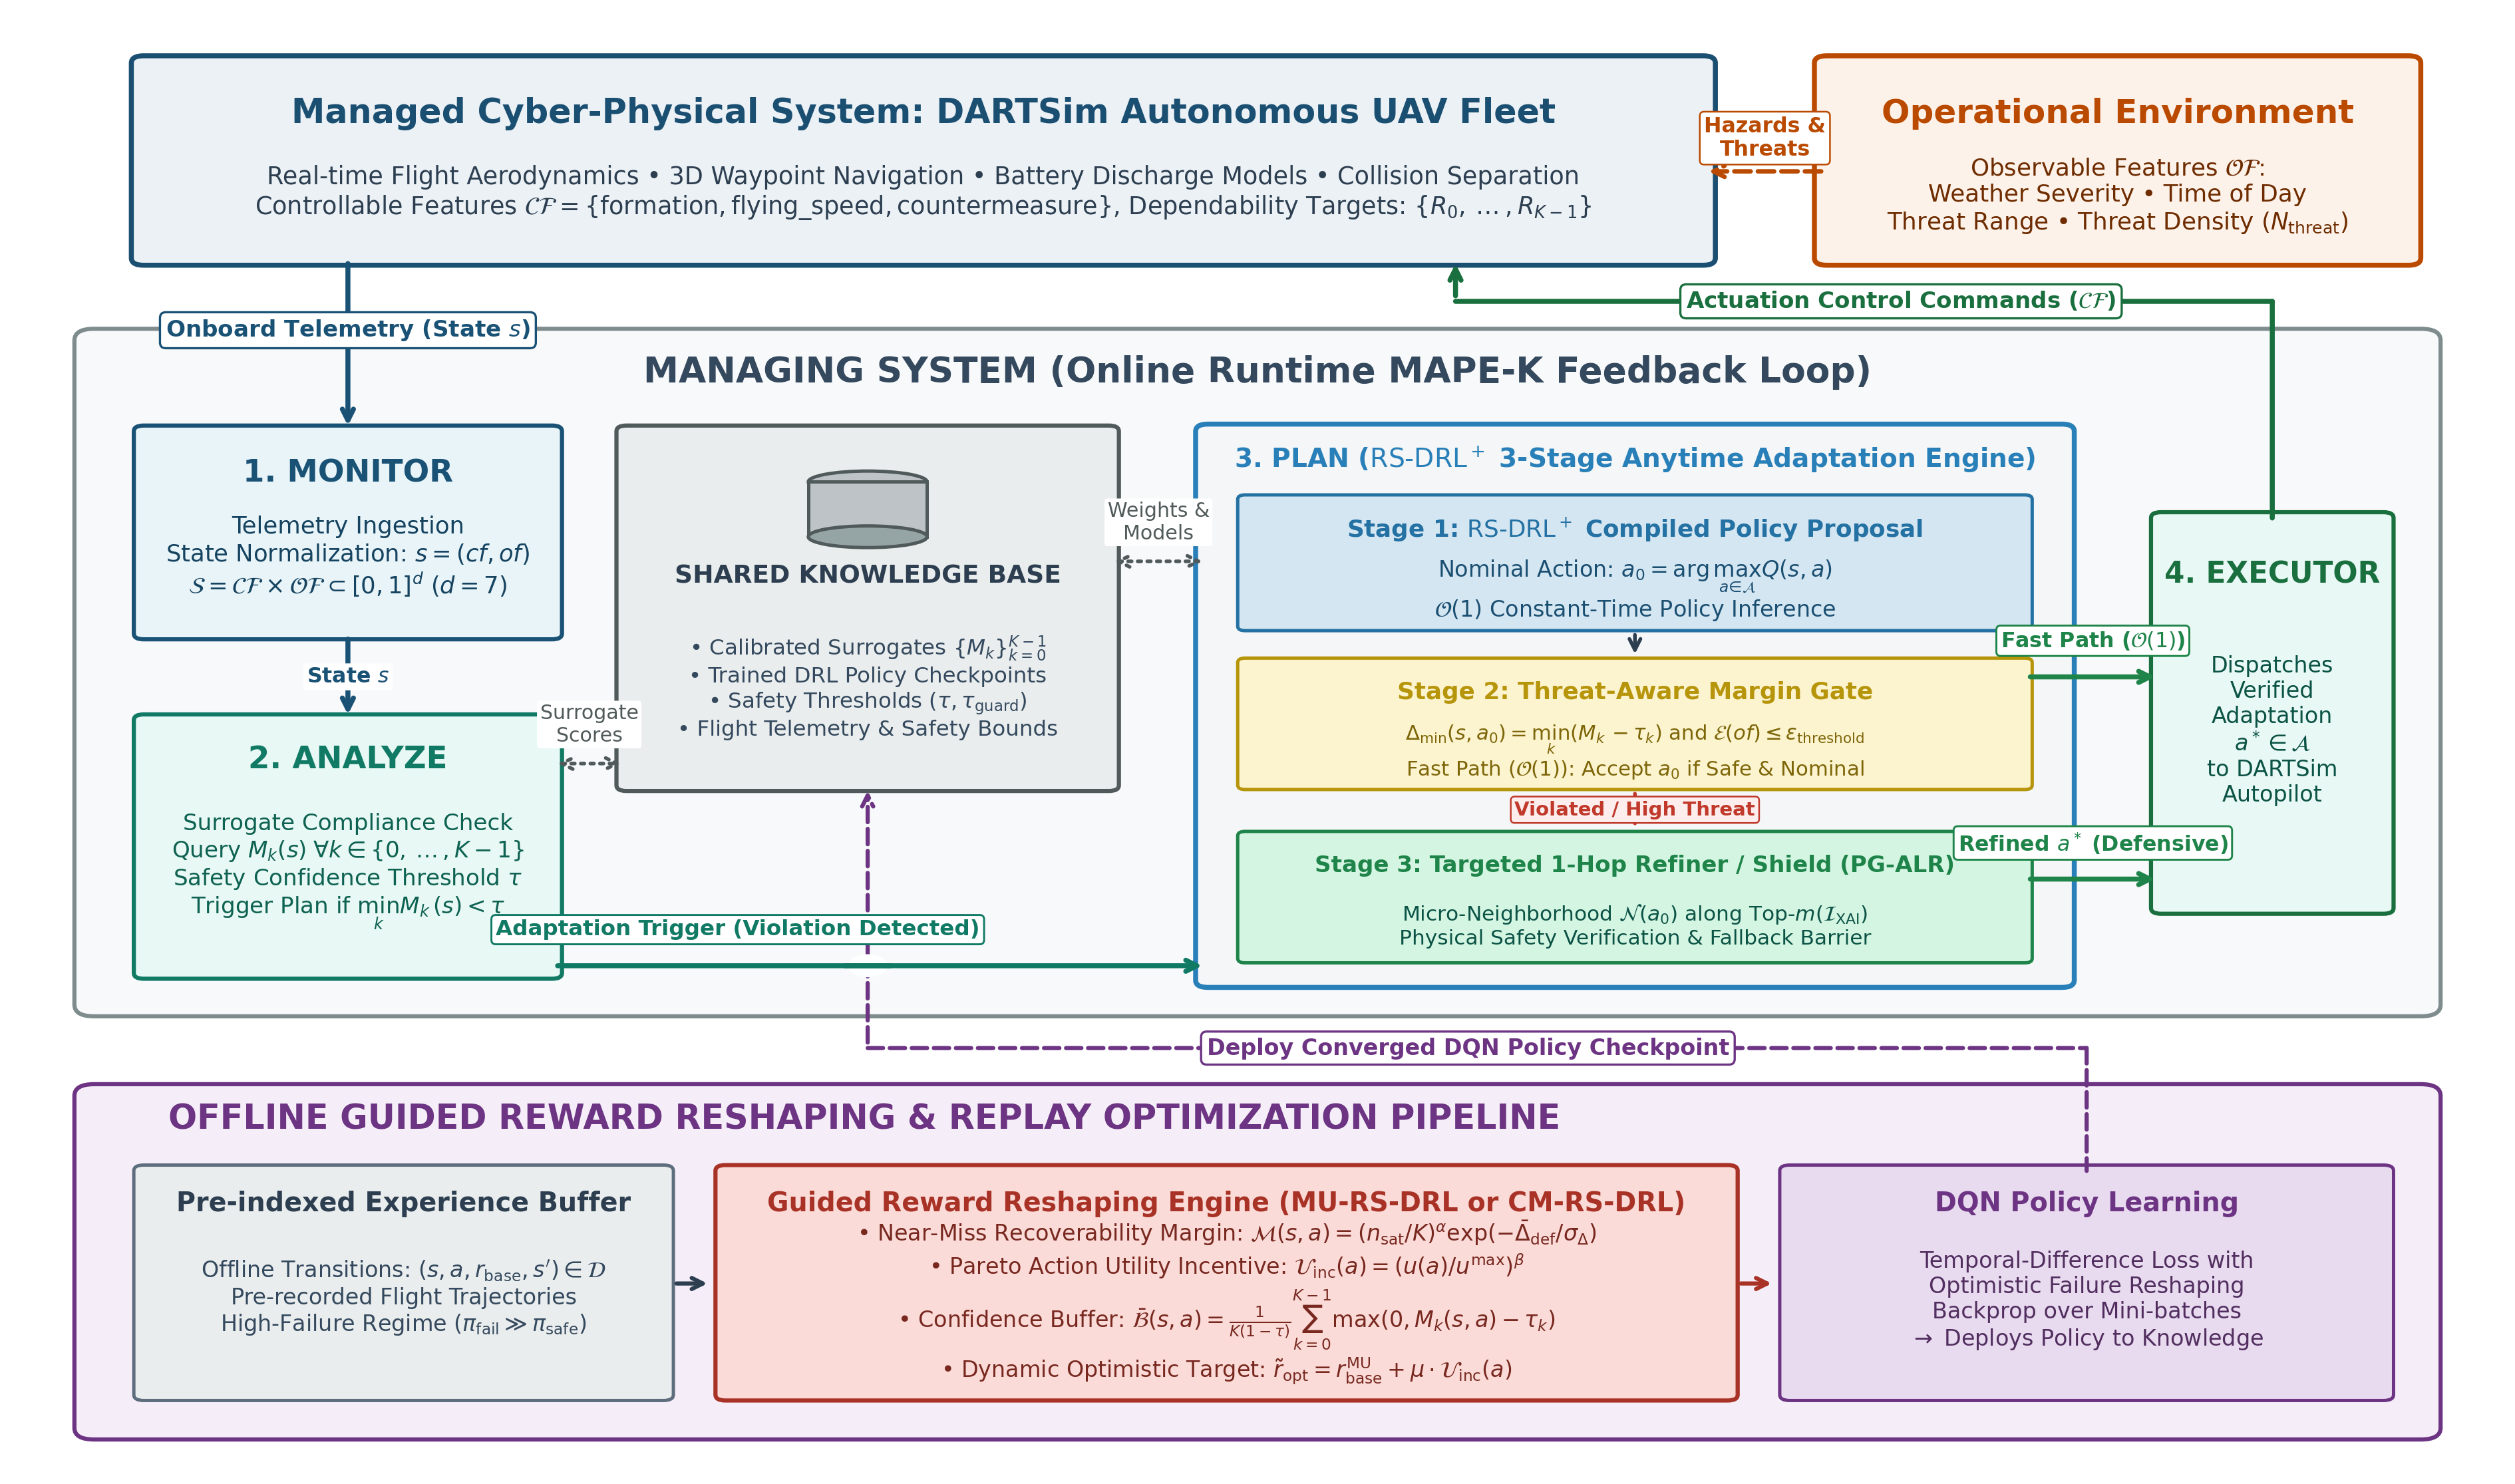
\includegraphics[width=0.95\textwidth]{figures/fig_system_architecture.png}
\caption{نمای کلان معماری دوسطحی \rsdrlplus: خط لوله آموزش آفلاین با شکل‌دهی پاداش حساس به حاشیه (سطح پایین)، و حلقه کنترلی \lr{MAPE-K} مجهز به برنامه‌ریز سلسله‌مراتبی سه‌مرحله‌ای \pgalr در سطح آنلاین برای کنترل ناوگان پهپادی \lr{DARTSim}.}
\label{fig:rsdrl_plus_system_architecture}
\end{figure*}

شکل \ref{fig:method_taxonomy_tree} درخت رده‌بندی روش‌های تصمیم‌گیری در سیستم‌های خودوفق را نشان می‌دهد که سیر تکاملی از روش‌های کلاسیک جستجو و سپرهای ایستا تا یادگیری تقویتی بدون هدایت، روش پایه‌ای \lr{RS-DRL} و در نهایت معماری جامع دوسطحی \rsdrlplus را تبیین می‌نماید.

\begin{figure}[htbp]
\centering
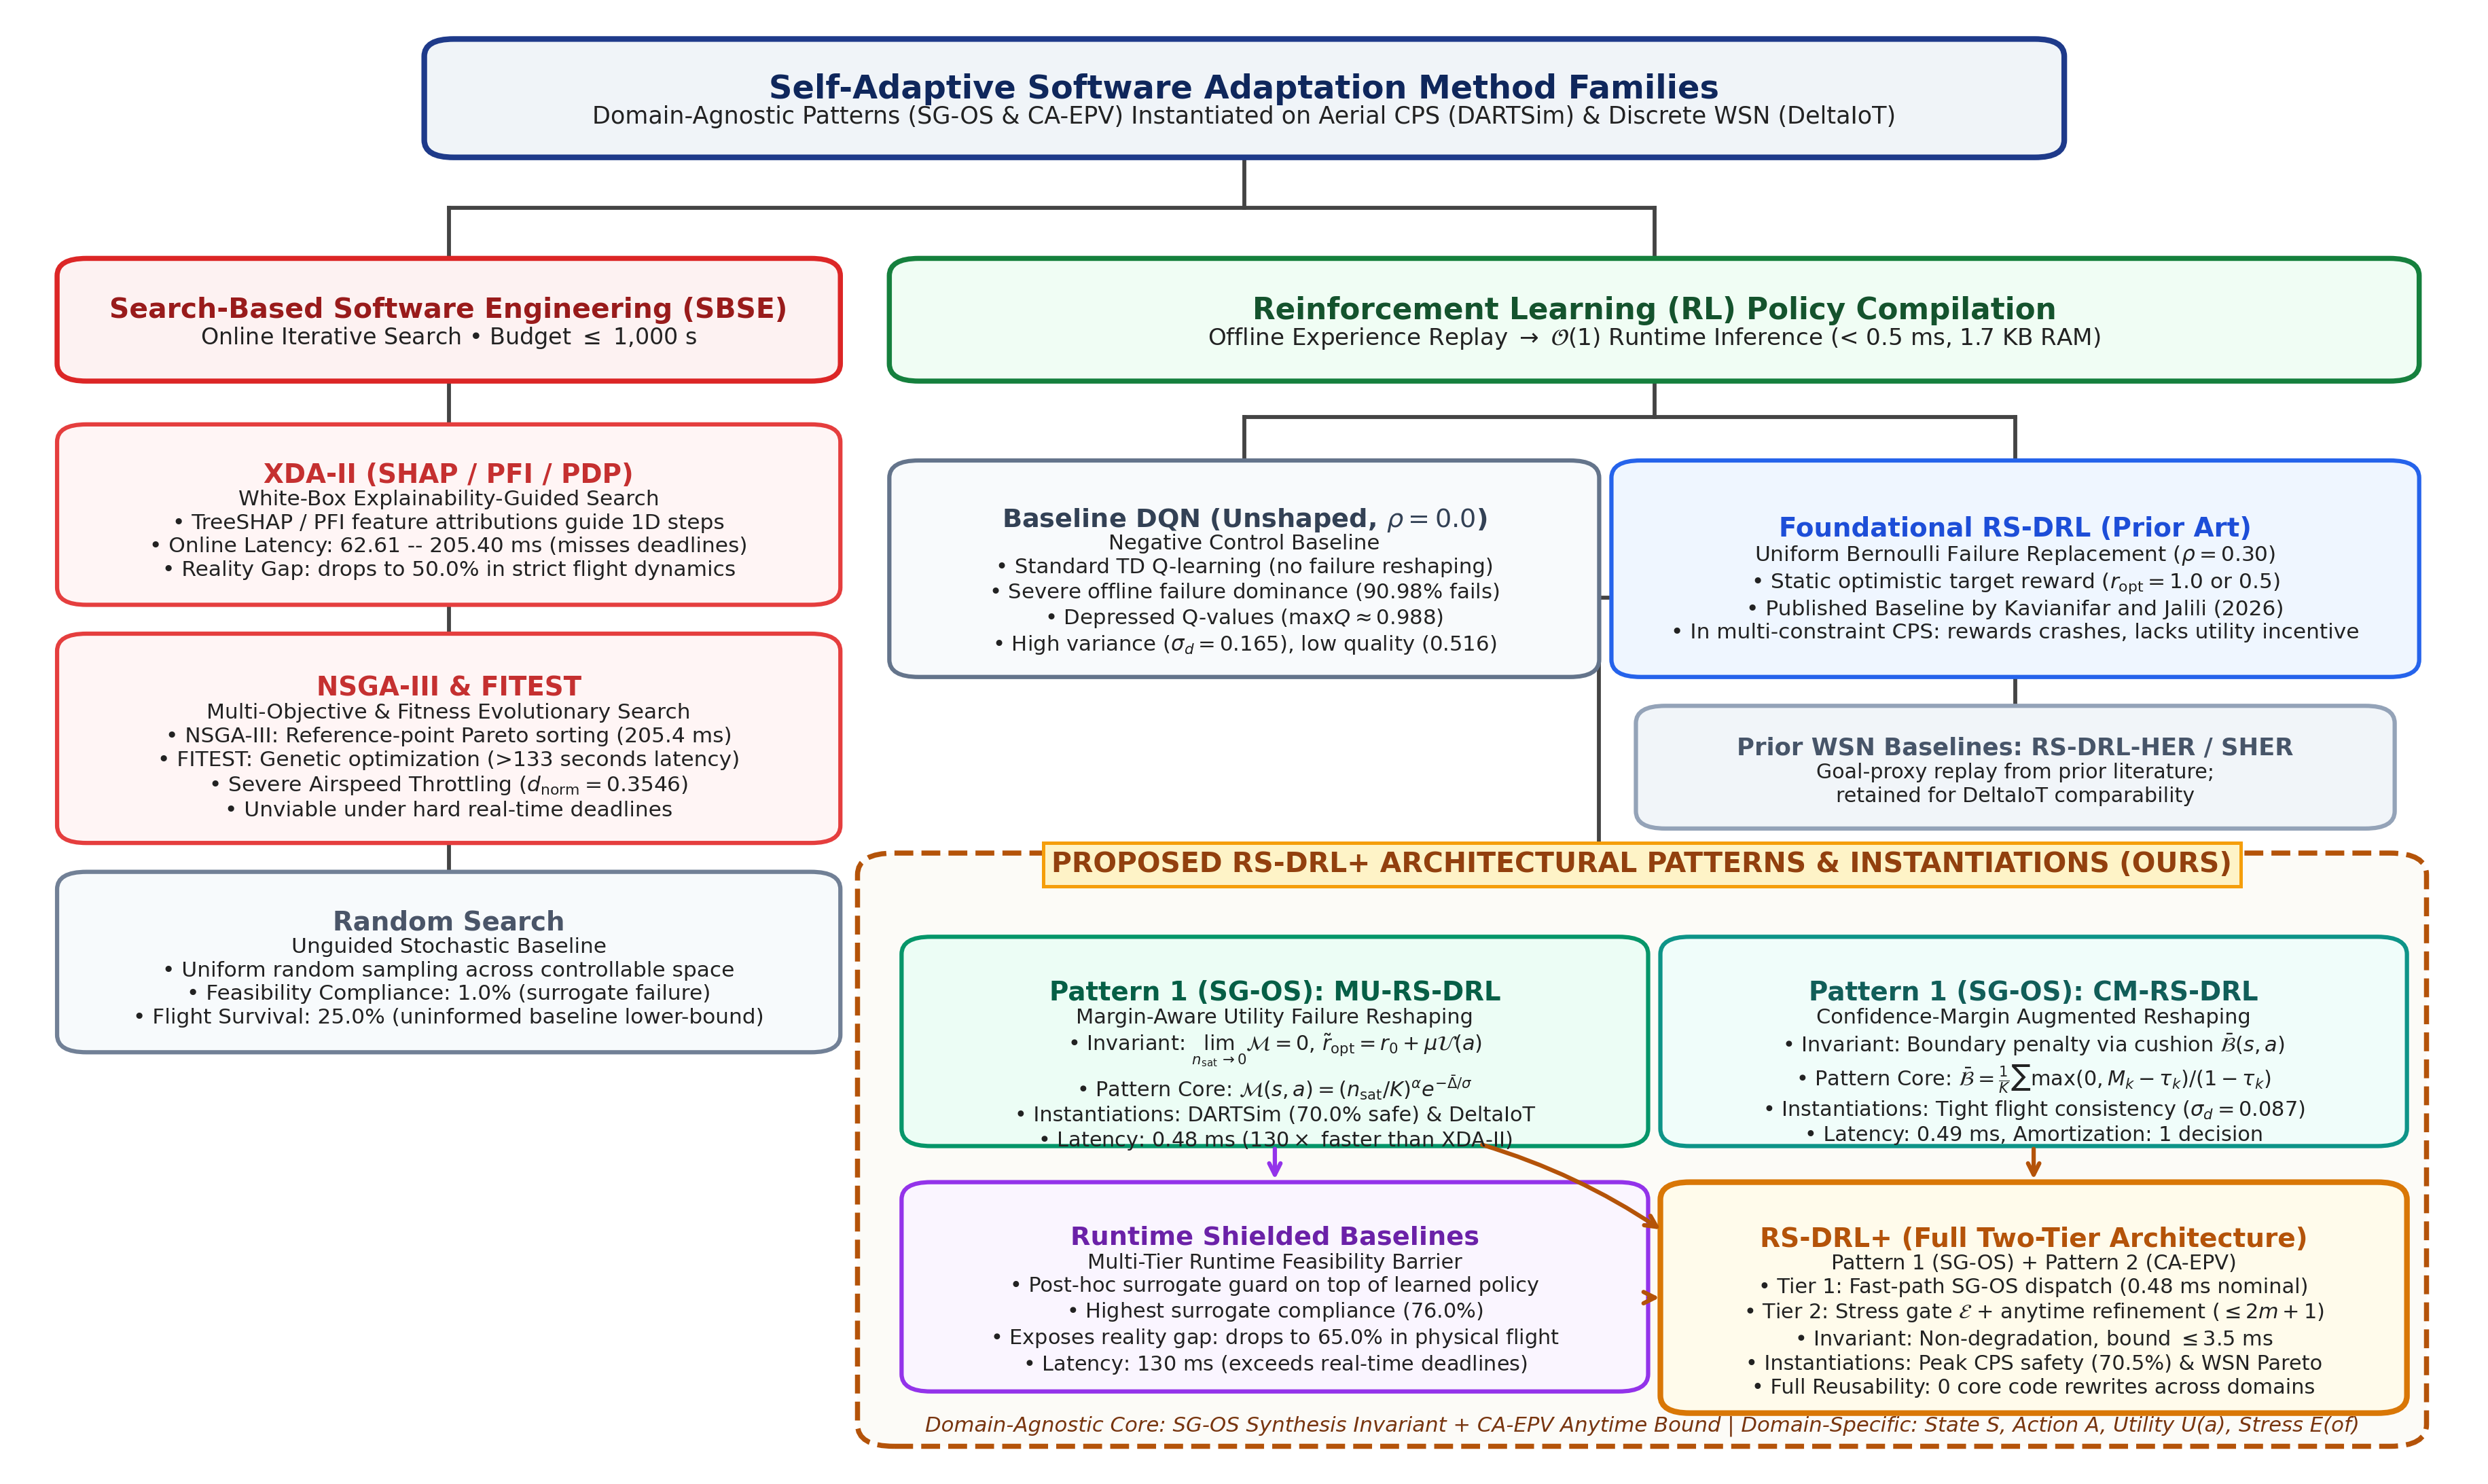
\includegraphics[width=0.88\linewidth]{figures/fig_method_taxonomy_tree.png}
\caption{درخت رده‌بندی و سیر تکاملی روش‌های تصمیم‌گیری در سیستم‌های خودوفق: از بهینه‌سازی مبتنی بر جستجو و سپرهای صوری ایستا تا یادگیری تقویتی عمیق بدون هدایت، روش پایه‌ای \lr{RS-DRL} و چارچوب دوسطحی تعمیم‌یافته \rsdrlplus.}
\label{fig:method_taxonomy_tree}
\end{figure}

\subsection{سطح آنلاین (\lr{Online Tier})}
در سطح آنلاین، حلقه \lr{MAPE-K} بر روی بردار حالت نرمال‌شده $s = (cf, of)$ و مدل‌های جانشین $M_k$ عمل می‌کند. مؤلفه تحلیل (\lr{Analyze}) در صورتی که حداقل یک قید به مرز هشدار نزدیک شود ($\min_k M_k(s) < \tau$) برنامه‌ریز را فعال می‌سازد. مؤلفه اجرا (\lr{Execute}) اقدام تطبیقی برگزیده شامل تنظیمات سرعت، آرایش تیمی و اقدامات متقابل الکترونیکی (\lr{ECM}) را اعمال می‌کند. مخزن دانش وزن‌های شبکه، آستانه‌ها و سوابق پرواز را ذخیره می‌سازد.

\subsection{سطح آفلاین (\lr{Offline Tier})}
در سطح آفلاین، بافر بازپخش تجارب $\mathcal{D}$ شامل ده‌ها هزار گذار ثبت‌شده $(s, a, r_{\text{base}}, s', d)$ است. در هر مینی‌بچ، فرآیند برچسب‌گذاری مجدد پاداش به صورت برنولی تحت احتمال هدایت‌شده $P_{\text{reshape}}$ اعمال می‌گردد. تابع زیان یادگیری تقویتی عمیق بر پایه خطای تفاضل زمانی خارج از سیاست (\lr{Off-Policy TD Loss}) به صورت زیر فرمول‌بندی می‌شود:
\begin{equation}
\label{eq:dqn_loss_rsdrlplus}
\mathcal{L}(\theta) = \mathbb{E}_{(s, a, \tilde{r}, s', d) \sim \mathcal{D}} \left[ \Big( \tilde{r} + (1 - d)\gamma \max_{a' \in \mathcal{A}} Q(s', a'; \theta^-) - Q(s, a; \theta) \Big)^2 \right]
\end{equation}
که در آن $\tilde{r}$ پاداش شکل‌یافته هدایت‌شده و $d \in \{0, 1\}$ نشان‌گر وضعیت پایانی است. در بستر مأموریت پهپادی \lr{DARTSim}، با تثبیت فاکتورهای محیطی و تغییر فاکتورهای کنترلی، هر تصمیم یک گام به عنوان وضعیت پایانی در نظر گرفته شده ($d=1$) که مسئله را به رگرسیون راهزن زمینه‌آگاه ۱-گام (\lr{Contextual Bandit}) تبدیل می‌کند و مانع از واگرایی ریاضی مقادیر کیو ($Q \to -\infty$) می‌گردد.

% =========================================================================
\section{الگوی اول: سنتز آفلاین هدایت‌شده با مشخصه‌ها (\texorpdfstring{\sgos}{SG-OS})}
\label{sec:sgos_pattern}
% =========================================================================

الگوی \sgos جایگزین نمونه‌برداری تصادفی یکنواخت پیشین شده و از مشخصه‌های صوری و حاشیه‌های کیفی برای هدایت فرآیند شکل‌دهی پاداش بهره می‌گیرد. این الگو از طریق دو مؤلفه \mursdrl و \cmrsdrl تحقق می‌یابد:

\subsection{شکل‌دهی پاداش هدایت‌شده با حاشیه بازیابی و مطلوبیت (\mursdrl)}
\label{subsec:mu_rs_drl_method}

روش \mursdrl از طریق چهار مؤلفه ریاضی صوری پیاده‌سازی می‌گردد:

\paragraph{۱. حاشیه بازیابی خطاهای نزدیک (\lr{Near-Miss Recoverability Margin}):}
برای هر گذار نقض‌کننده الزامات $(s, a)$، میزان نزدیکی پیکربندی به انطباق کامل با رابطه ریاضی زیر سنجیده می‌شود:
\begin{equation}
\label{eq:recoverability_margin}
\mathcal{M}(s, a) = \left( \frac{n_{\text{sat}}}{K} \right)^\alpha \exp\left( - \frac{\bar{\Delta}_{\text{def}}(s, a)}{\sigma_\Delta} \right)
\end{equation}
که در آن $K$ تعداد کل الزامات کیفی (۱۲ در \lr{DARTSim})، $n_{\text{sat}}$ تعداد الزامات ارضاشده، $\alpha \ge 1$ توان جریمه نقض هم‌زمان چند قید، $\bar{\Delta}_{\text{def}}$ میانگین کسری اطمینان تا آستانه‌ها، و $\sigma_\Delta > 0$ فاکتور مقیاس خطای کسری است.

از منظر مفهومی، این فرمولاسیون دو بعد مجزا از خطا را ادغام می‌نماید: \textbf{پهنای شکست} ($n_{\text{sat}}/K$) که نشان‌دهنده تعداد قیود نقض‌شده است، و \textbf{عمق شکست} ($\bar{\Delta}_{\text{def}}$) که شدت تخطی از حاشیه آستانه‌ها را منعکس می‌کند. اگر چندین قید به طور هم‌زمان نقض گردند، عبارت توان‌دار به شدت افت کرده (به عنوان مثال با $\alpha=2$ و ارضای نصف قیود، به $0.25$ کاهش می‌یابد) و با تعمیق انحراف از آستانه‌ها، ضریب نمایی نیز به صفر میل می‌کند. بنابراین، شکست‌های فاجعه‌بار و چندگانه به طور قطعی پالایش شده و هرگز پاداش مصنوعی دریافت نمی‌کنند ($\lim_{n_{\text{sat}} \to 0} \mathcal{M} = 0$).

\paragraph{۲. مشوق مطلوبیت عملیاتی اقدام (\lr{Action Utility Incentive}):}
به منظور مهار پدیده «ایمنی ناشی از انفعال» (\lr{Safety through Inaction Trap}) که در آن عامل برای اجتناب از نقض قیود راداری به مدهای غیرعملیاتی (نظیر توقف در فاصله دور از اهداف شناسایی) پناه می‌برد، مشوق مطلوبیت اقدام تعریف می‌گردد:
\begin{equation}
\label{eq:utility_incentive}
\mathcal{U}_{\text{inc}}(a) = \left( \frac{u(a)}{u^{\max}} \right)^\beta
\end{equation}
که در آن $u(a)$ مطلوبیت مأموریت (نظیر فاصله نرمال‌شده تا هدف $d_{\text{norm}}$ در پهپاد، یا مطلوبیت شبکه $\mathcal{U}_{\text{WSN}}$ در حسگر بی‌سیم) و $\beta = 1.0$ فاکتور مقیاس است.

\paragraph{۳. احتمال شکل‌دهی هدایت‌شده (\lr{Guided Reshaping Probability}):}
گذار ناموفق با احتمالی متناسب با حاشیه بازیابی و مطلوبیت با پاداش خوش‌بینانه جایگزین می‌گردد:
\begin{equation}
\label{eq:guided_prob}
P_{\text{reshape}}(s, a) = \rho_{\text{base}} \cdot \mathcal{M}(s, a) \cdot \left[ (1 - \gamma_u) + \gamma_u \mathcal{U}_{\text{inc}}(a) \right]
\end{equation}
که در آن $\rho_{\text{base}} = 0.65$ سقف احتمال بازطراحی و $\gamma_u = 0.40$ وزن موازنه میان قابلیت بازیابی و مطلوبیت است.

\paragraph{۴. پاداش خوش‌بینانه دینامیک مقیاس‌بندی‌شده (\lr{Dynamic Optimistic Target}):}
برخلاف روش پایه‌ای که همواره پاداش ثابت $1.0$ تزریق می‌کرد، روش \mursdrl پاداش خوش‌بینانه را متناسب با مطلوبیت اقدام مقیاس‌بندی می‌کند:
\begin{equation}
\label{eq:dynamic_ropt}
\tilde{r}_{\text{opt}}(s, a) = r_{\text{base}}^{\text{MU}} + \mu \cdot \mathcal{U}_{\text{inc}}(a)
\end{equation}
که در آن $r_{\text{base}}^{\text{MU}} = 0.30$ و $\mu = 0.40$ است، به طوری که پاداش در بازه پیوسته $[0.30, 0.70]$ قرار می‌گیرد. شکل \ref{fig:failure_selection_mechanism} تفاوت بنیادین این سازوکار هدایت‌شده را با روش پایه‌ای نشان می‌دهد.

\begin{figure}[htbp]
\centering
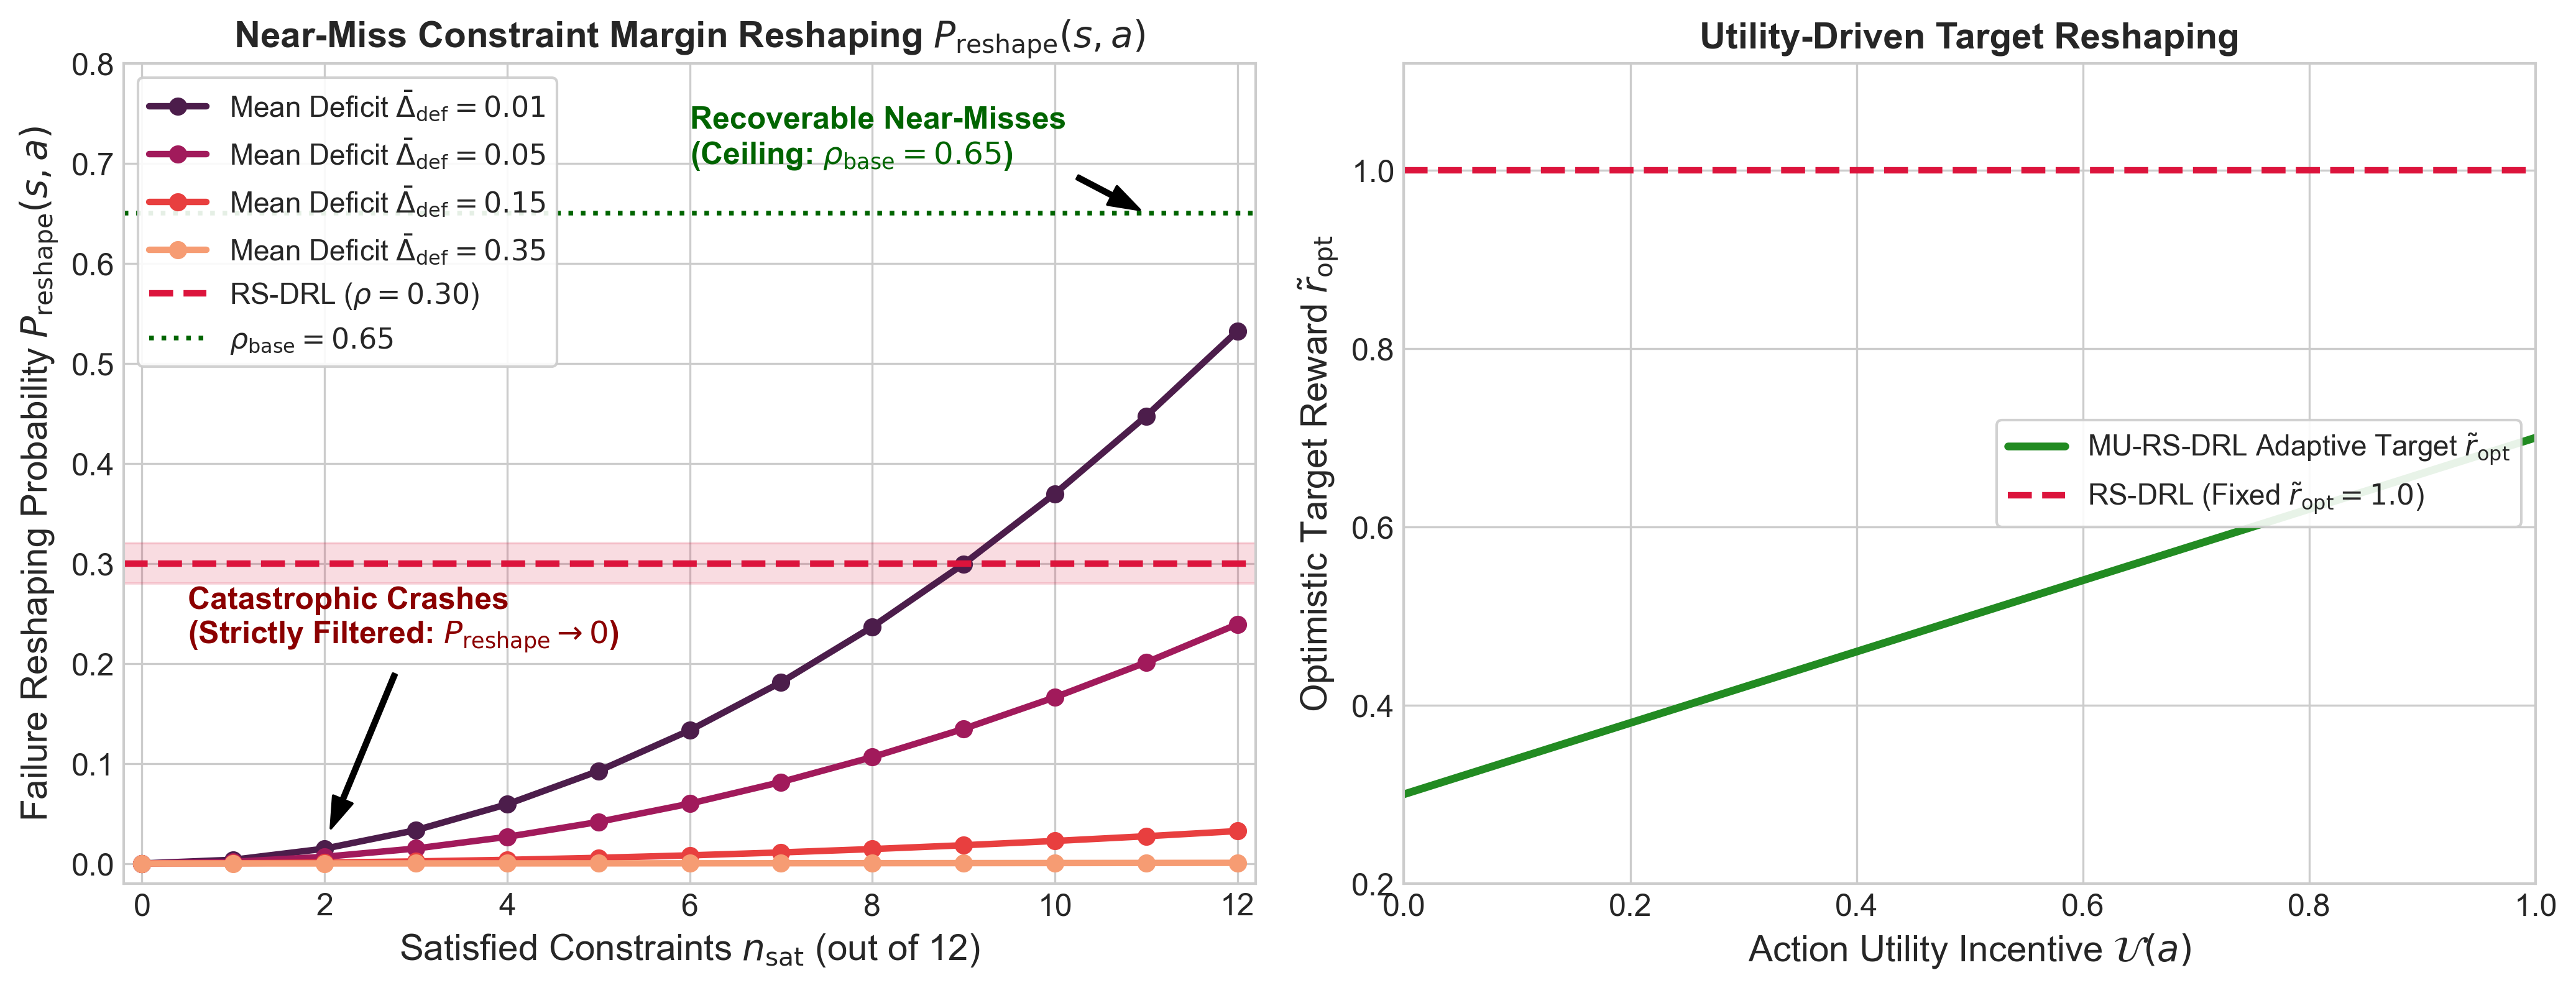
\includegraphics[width=0.90\linewidth]{figures/fig_failure_selection_mechanism.png}
\caption{مقایسه سازوکار شکل‌دهی پاداش در \mursdrl در برابر \lr{RS-DRL} پایه‌ای: (الف) تغییر پیوسته احتمال بر اساس تعداد الزامات ارضاشده و حاشیه بازیابی؛ (ب) مقیاس‌بندی پاداش خوش‌بینانه متناسب با مطلوبیت مأموریت.}
\label{fig:failure_selection_mechanism}
\end{figure}

\subsection{بافرسازی حاشیه اطمینان برای پایداری در مرزها (\cmrsdrl)}
\label{subsec:cm_rs_drl_method}

در سیستم‌های آستانه‌محور متداول ($M_k \ge \tau_k$)، تصمیمی که در مجاورت کرانی آستانه پذیرش قرار دارد پاداشی هم‌ارز با تصمیمات دارای حاشیه محافظه‌کارانه بالا دریافت می‌دارد. این پدیده منجر به شکنندگی سیاست کنترلی در برابر نوسانات تصادفی محیطی می‌گردد. جهت مدیریت این ناپایداری مرزی، رویکرد \cmrsdrl بافر حاشیه اطمینان نرمال‌شده را به شرح زیر محاسبه می‌نماید:
\begin{equation}
\label{eq:norm_conf_buffer}
\bar{\mathcal{B}}(s, a) = \frac{1}{K(1 - \tau)} \sum_{k=0}^{K-1} \max\big( 0, M_k(s, a) - \tau_k \big) \in [0, 1]
\end{equation}
که در آن $M_k(s, a)$ برآورد اطمینان قید $k$-ام و $\tau_k$ آستانه پذیرش متناظر است.

با استناد به این بافر اطمینان، سیگنال پاداش ایمن و پاداش شکل‌یافته با ضرایب وزن‌دهی $\lambda_{\text{margin}}$ و $\lambda_{\text{util}}$ بازنویسی و تقویت می‌شوند:
\begin{align}
r_{\text{safe}}(s, a) &= 1.0 + \lambda_{\text{margin}} \bar{\mathcal{B}}(s, a) + \lambda_{\text{util}} \mathcal{U}_{\text{inc}}(a) \label{eq:r_safe_cm} \\
\tilde{r}_{\text{CM}}(s, a) &= r_{\text{base}}^{\text{CM}} + \lambda_{\text{margin}} \bar{\mathcal{B}}(s, a) + \lambda_{\text{util}} \mathcal{U}_{\text{inc}}(a) \label{eq:r_cm_reshaped}
\end{align}
این تزریق حاشیه صریح تضمین می‌کند که سیاست یادگیرنده از گزینه‌های لب‌مرزی که در مواجهه با تلاطم‌های جوی و نویز باد ناپایدار می‌شوند دوری جسته و به سمت مناطق عملیاتی عمیقاً امن همگرا گردد.

% =========================================================================
\section{الگوی دوم: اعتبارسنجی کشسان با قرارداد در هر زمان (\texorpdfstring{\caepv}{CA-EPV})}
\label{sec:caepv_pattern}
% =========================================================================

الگوی \caepv در مؤلفه برنامه‌ریزی (\lr{Plan}) درون ماژول پالایش موضعی هدایت‌شده با سیاست (\pgalr) استقرار یافته و فرآیند تصمیم‌گیری را در سه مرحله سازماندهی می‌نماید:

\subsection{سلسله‌مراتب تصمیم‌گیری سه‌مرحله‌ای}

\paragraph{مرحله اول: استنتاج پیشنهاد نامی زیر میلی‌ثانیه‌ای ($0.485\text{ms}$):}
برنامه‌ریز با یک گذر رو به جلوی فوق‌سریع در شبکه عصبی آموزش‌دیده $Q_{\text{MU}}$، گزینه نامی بهینه $a_0 = \arg\max_{a} Q_{\text{MU}}(s, a)$ را در زمان میانگین $0.485\text{ms}$ پیشنهاد می‌دهد.

\paragraph{مرحله دوم: گیت حاشیه و شدت تنش محیطی (\lr{Fast Path}):}
پیشنهاد نامی وارد یک گیت اعتبارسنجی سریع می‌شود که حاشیه مدل جانشین و شدت تنش محیطی را با رابطه زیر ارزیابی می‌کند:
\begin{equation}
\label{eq:margin_gate}
\Delta_{\min}(s, a_0) = \min_{k} \big( M_k(s, a_0) - \tau_k \big), \qquad \mathcal{E}(of) = \sum_{j=1}^{|\mathcal{OF}|} w_j \cdot \widetilde{of}_j
\end{equation}
در صورتی که $\Delta_{\min}(s, a_0) \ge 0$ و شدت تنش محیطی زیر آستانه بحرانی باشد ($\mathcal{E}(of) \le \epsilon_{\text{threshold}}$)، گزینه نامی بلافاصله در «مسیر سریع» (\lr{Fast Path}) بدون هیچ تأخیری به عملگرها ارسال می‌گردد (تأخیر کل زیر $0.5\text{ms}$).

\paragraph{مرحله سوم: پالایش دفاعی ۱-گام هدفمند مبتنی بر \lr{XAI}:}
در صورت نقض هر یک از شرایط فوق، پالایش موضعی پیرامون $a_0$ فعال می‌گردد. برای جلوگیری از انفجار محاسباتی، پالایش بر روی زیرفضای حساسیت حاصل از مقادیر شاپلی درختی (\lr{TreeSHAP}) متمرکز می‌شود:
\begin{equation}
\label{eq:shap_projection}
\mathcal{I}_{\text{XAI}}(j) = \frac{1}{K} \sum_{k=0}^{K-1} \mathbb{E}_{s \sim \mathcal{D}} \big[ |\phi_j(M_k, s)| \big]
\end{equation}
همسایگی مجاز کاندیداها به گام‌های ۱-سطحی روی $m$ ویژگی برتر محدود می‌گردد:
\begin{equation}
\label{eq:xai_neighborhood}
\begin{aligned}
\mathcal{N}(a_0) = \bigg\{ a \in \mathcal{A} \;\bigg|\; &\forall j \notin \text{Top-}m(\mathcal{I}_{\text{XAI}}),\, k_j(a) = k_j(a_0) \\
&\land\; \sum_{j \in \text{Top-}m} |k_j(a) - k_j(a_0)| \le 1 \bigg\}
\end{aligned}
\end{equation}
شکل \ref{fig:decision_hierarchy_flowchart} نمودار جریان تصمیم‌گیری این ساختار سلسله‌مراتبی را نشان می‌دهد.

\begin{figure}[htbp]
\centering
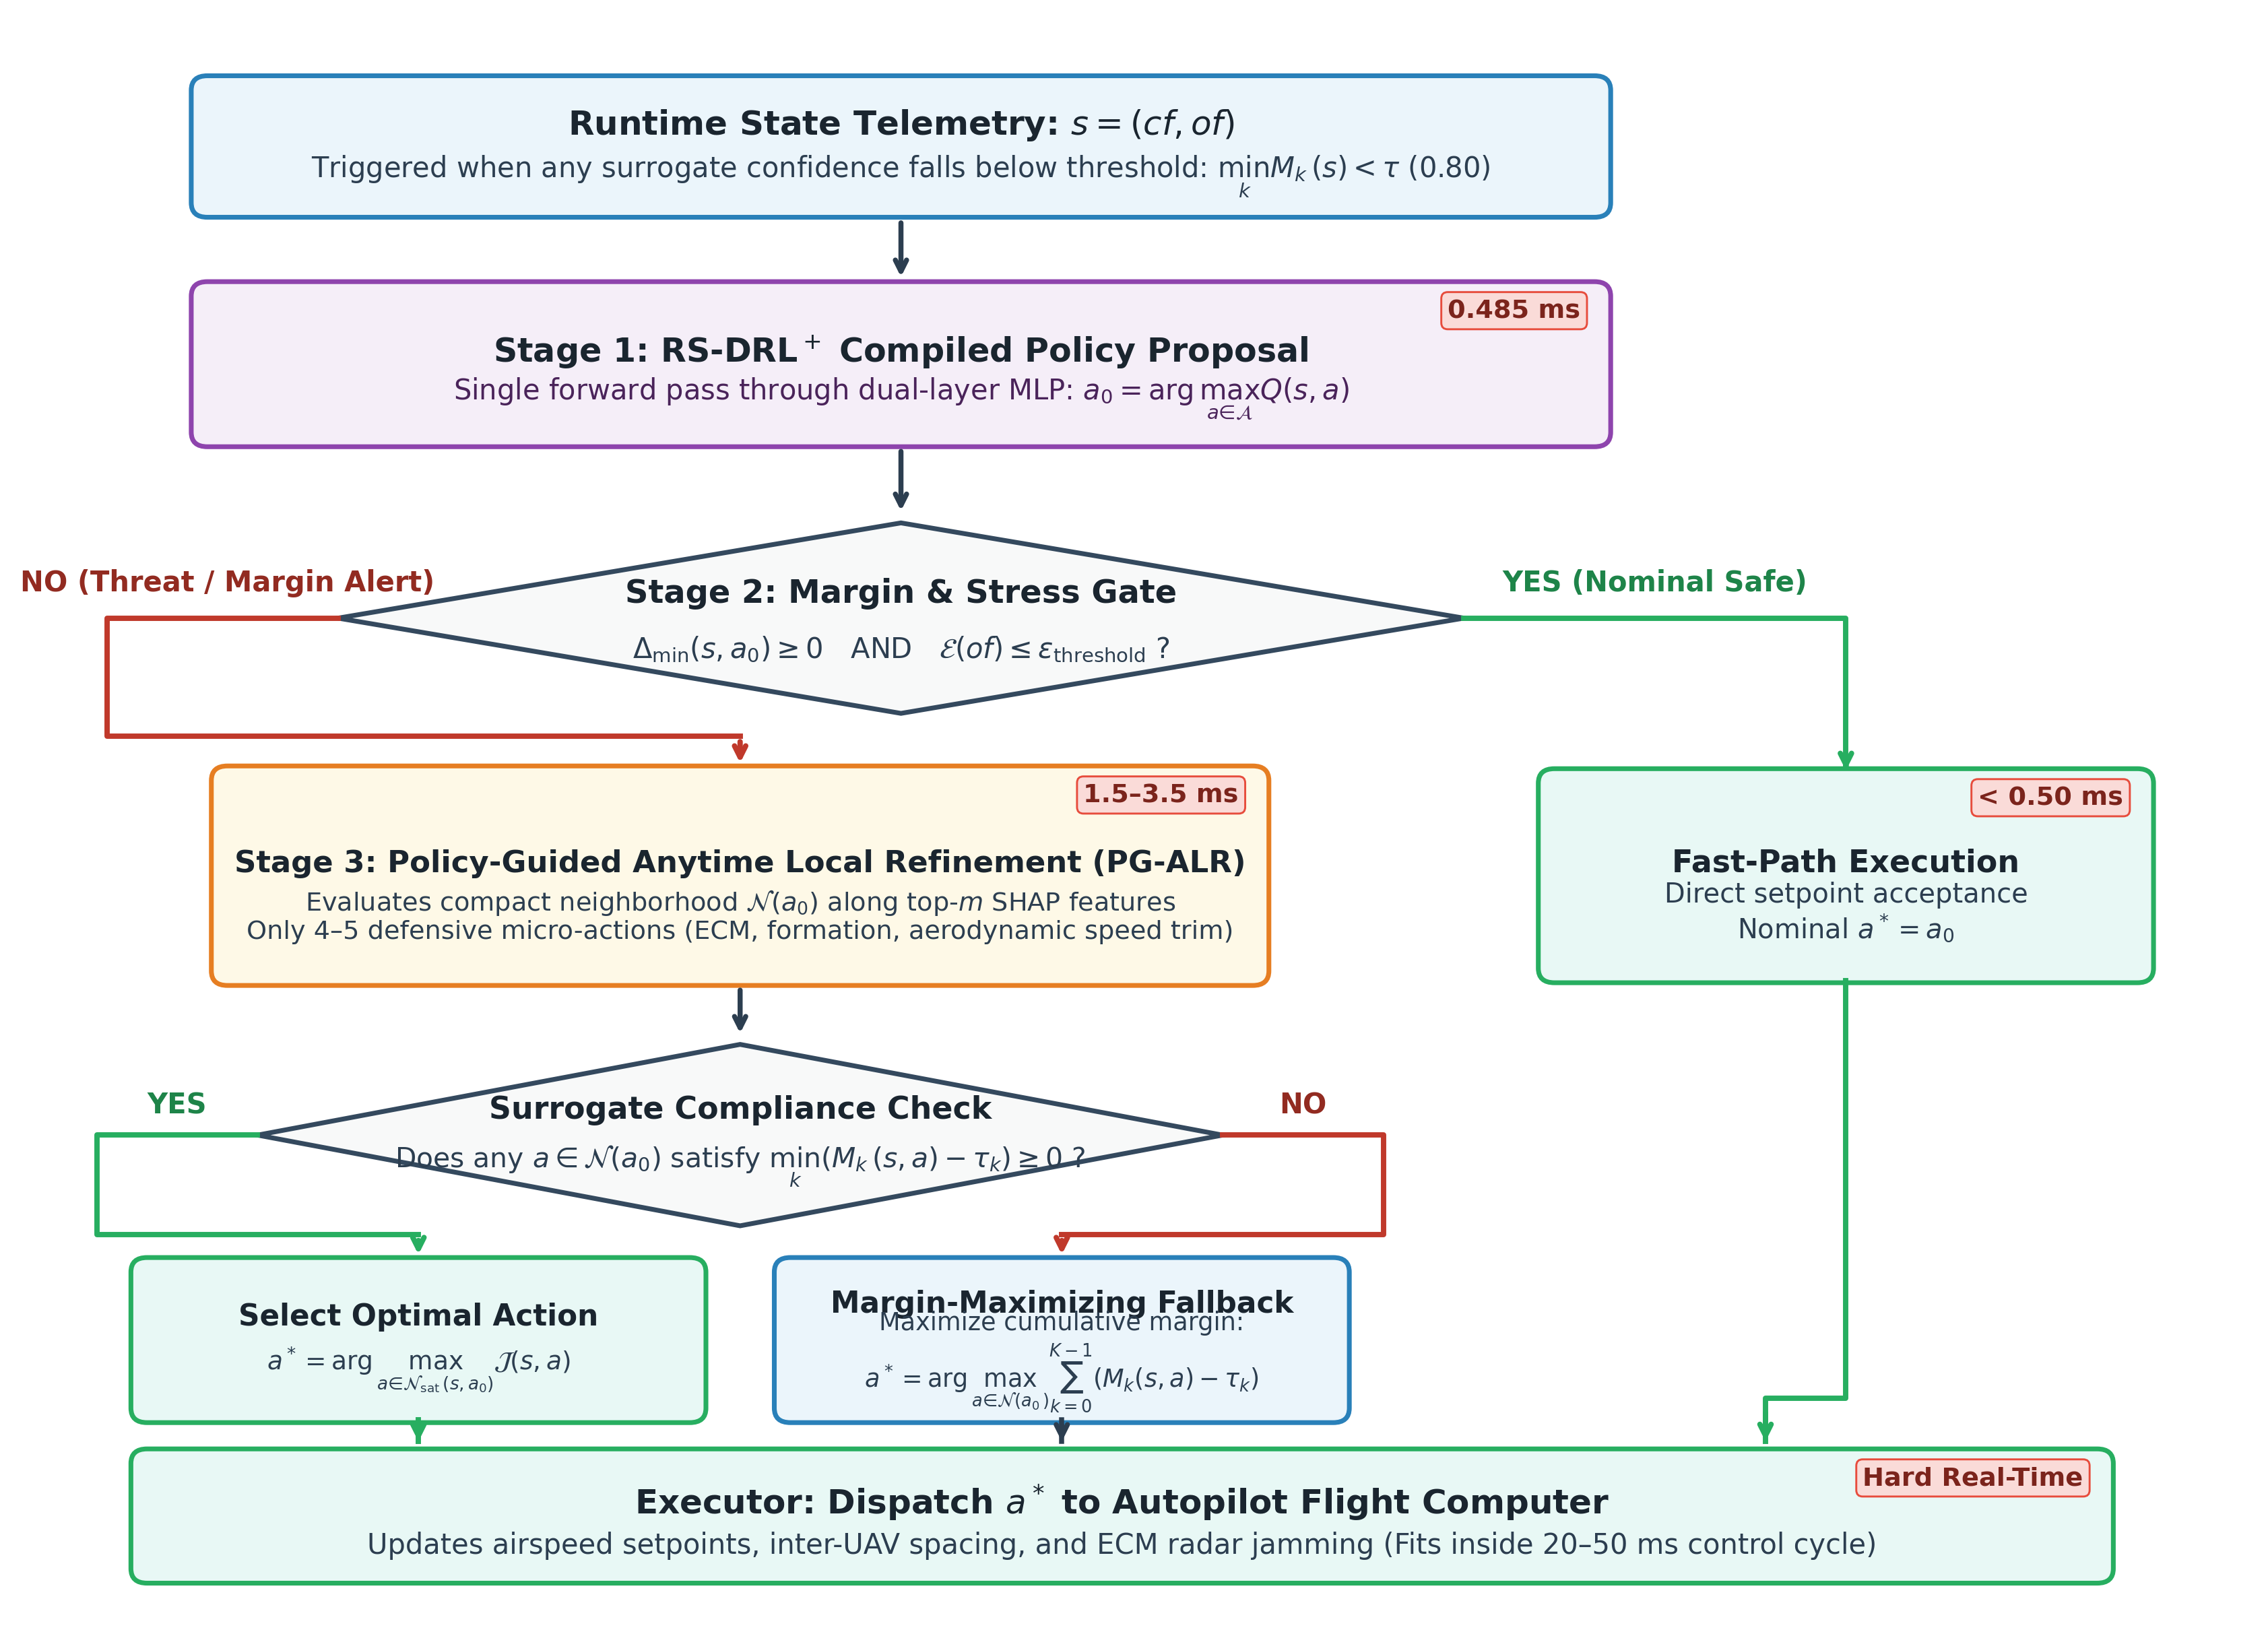
\includegraphics[width=0.88\linewidth]{figures/fig_decision_hierarchy_flowchart.png}
\caption[نمودار جریان سلسله‌مراتب تصمیم‌گیری ماژول \pgalr]{نمودار جریان سلسله‌مراتب تصمیم‌گیری ماژول \pgalr: استنتاج نامی مرحله ۱ ($0.485\text{ms}$)، گیت تنش مرحله ۲، پالایش موضعی ۱-گام مرحله ۳ ($1.5-3.5\text{ms}$) و سازوکار فال‌بک حداکثرسازی حاشیه.}
\label{fig:decision_hierarchy_flowchart}
\end{figure}

\subsection{تضمین‌های صوری و تحلیل ریاضی پیچیدگی}

\begin{proposition}[کران کاردینالیتی تصویرشده بر حساسیت]
\label{prop:complexity_bound}
برای هر پیشنهاد نامی $a_0 \in \mathcal{A}$ در فضای پیکربندی گسسته با ابعاد $d_A$ با مؤلفه‌های ترتیبی یا دودویی، محدودسازی اغتشاشات به گام‌های ۱-سطحی بر روی $m$ ویژگی حساسیت برتر ($m \le d_A$)، مجموعه‌ای از کاندیداها به دست می‌دهد که اندازه آن توسط نامساوی زیر مقید است:
\begin{equation}
\label{eq:complexity_bound}
|\mathcal{N}(a_0)| \le 2m + 1
\end{equation}
در صورتی که هر یک از ویژگی‌ها در مرزهای بازه مقداری خود قرار داشته باشند، نامساوی اکید خواهد بود.
\end{proposition}

\begin{proof}
کاندیدای نامی $a_0$ دارای فاصله مختصاتی صفر است. برای هر بعد $j \in \{1, \dots, m\}$ از ویژگی‌های تصویرشده، حداکثر دو اغتشاش ۱-گامی مجاز وجود دارد: افزایش یک سطح ($+1$) یا کاهش یک سطح ($-1$). طبق تعریف معادله \ref{eq:xai_neighborhood}، مجموع فواصل مختصاتی اغتشاش‌ها نباید از ۱ تجاوز کند؛ بنابراین، هیچ دو بعدی نمی‌توانند به طور همزمان تغییر کنند. با جمع بستن تعداد تغییرات مجاز روی تمامی $m$ بعد، حداکثر $2m$ همسایه مجزا حاصل می‌گردد. با افزودن خود نقطه مبدأ $a_0$، حداکثر تعداد اعضای همسایگی برابر با $2m + 1$ خواهد بود. در صورت برخورد هر بعد به کران‌های کمینه یا بیشینه فیزیکی، امکان حرکت در آن جهت سلب شده و کاردینالیتی اکیداً کمتر از $2m + 1$ می‌گردد.
\end{proof}

\paragraph{اهمیت معماری گزاره ۱:}
این گزاره اثبات می‌کند که پیچیدگی اعتبارسنجی زمان اجرا از مرتبه نمایی کل فضای پیکربندی $\mathcal{O}(|\mathcal{A}| \cdot K)$ به مرتبه خطی متغیرهای حساس $\mathcal{O}(m \cdot K)$ کاهش می‌یابد. در ناوگان پهپادی \lr{DARTSim} ($m=3$)، تعداد گزینه‌های مورد ارزیابی از ۶۰ پیکربندی به حداکثر ۴ تا ۵ گزینه کاهش می‌یابد (کاهش ۹۳٪ در ارزیابی‌ها). این کران ریاضی تضمین می‌کند که زمان اعتبارسنجی همواره زیر $3.5\text{ms}$ باقی مانده و مهلت زمانی ۲۰ تا ۵۰ میلی‌ثانیه سیستم کنترل پرواز به طور قطعی ارضا گردد.

\paragraph{پیچیدگی محاسباتی و موازی‌سازی تانسوری (\lr{Tensorized Parallelism}):}
با داشتن $K$ مدل جانشین ارزیابی ایمنی $M_0, \dots, M_{K-1}$، اعتبارسنجی در هر زمان نیازمند محاسبه بردار انطباق بر روی کاندیداهای همسایگی $\mathcal{N}(a_0)$ است:
\begin{equation}
\label{eq:compliance_vector}
\mathbf{P}(a) = \big[ M_0(s, a),\, \dots,\, M_{K-1}(s, a) \big] \in [0, 1]^K
\end{equation}
بر اساس گزاره \ref{prop:complexity_bound}، تعداد کل ارزیابی‌های زوج کاندیدا-مدل جانشین توسط نامساوی زیر مقید است:
\begin{equation}
\label{eq:tensor_eval_bound}
N_{\text{eval}} \le (2m + 1) \cdot K
\end{equation}
در پیاده‌سازی ناوگان پهپادی \lr{DARTSim} با ابعاد کنترلی $d_A = 3$، پارامتر حساسیت $m = 3$ و تعداد الزامات $K = 12$، کران تئوریک برابر با $N_{\text{eval}} \le (2 \times 3 + 1) \times 12 = 84$ ارزیابی است. در زمان اجرا، به دلیل اشباع مرزهای فیزیکی پارامترها، کاندیداهای معتبر به ۴ تا ۵ پیکربندی فیلتر شده و تعداد ارزیابی‌ها به ۴۸ تا ۶۰ کاهش می‌یابد.

از منظر پیاده‌سازی سخت‌افزاری، از آنجا که تانسور کاندیداها $\mathbf{A}_{\text{cand}} \in \mathbb{R}^{|\mathcal{N}(a_0)| \times d_A}$ بلافاصله پس از استنتاج نامی به صورت قطعی مشخص است، ارزیابی بر روی تمامی مدل‌های جانشین در قالب یک بچ موازی تانسوری (\lr{SIMD}) بر روی پردازنده‌های استاندارد بدون نیاز به شتاب‌دهنده گرافیکی در زمان ۱/۵ تا ۳/۵ میلی‌ثانیه انجام می‌پذیرد. این در حالی است که سپرهای ایمنی زمان اجرای کلاسیک نیازمند ۷۲۰ ارزیابی برخط ($60 \times 12$) و صرف زمان ۱۲۹/۹۵ میلی‌ثانیه هستند؛ بنابراین، روش پیشنهادی با ایجاد شتاب‌بخشی بیش از ۴۰ برابری، پایداری مهلت زمانی ۲۰ تا ۵۰ میلی‌ثانیه‌ای خلبان خودکار را به طور قطعی تضمین می‌نماید.

\paragraph{تحلیل مقیاس‌پذیری در فضاهای با ابعاد بالا ($d_A \gg 1$) در برابر فضاهای گسسته شبکه‌ای:}
در سیستم‌های خودوفق با ابعاد متغیرهای کنترلی بسیار بزرگ (نظیر بستر \lr{DeltaIoT} با $d_A = 37$ گره حسگر)، یک اغتشاش ۱-گامی چندمحوره نامقید در فضای $L_\infty$ به صورت توان‌نمایی $3^{d_A}$ رشد می‌کند؛ این مقدار برای ۳۷ گره معادل $3^{37} \approx 4.5 \times 10^{17}$ پیکربندی است که هرگونه ارزیابی برخط را ناممکن می‌سازد. حتی اغتشاش تک‌محوره در نرم $L_1$ نیازمند ارزیابی $2d_A + 1 = 75$ گزینه است که فراتر از آستانه مجاز تأخیر بلادرنگ قرار می‌گیرد.

برای مهار این انفجار ترکیبیاتی، تصویرسازی هوش مصنوعی توضیح‌پذیر \lr{TreeSHAP} بر روی زیرفضای حساسیت $\mathcal{S}_{\text{XAI}} = \text{span}\{e_{j_1}, \dots, e_{j_m}\}$ استقرار می‌یابد. این تصویرسازی ابعاد تصمیم‌گیری را از $d_A$ به $m \ll d_A$ (به عنوان مثال $m = 3 \ll 37$) کاهش داده و ارزیابی‌ها را به طور قطعی به حداکثر $2m + 1 \le 7$ کاندیدای گلوگاهی مقید می‌سازد. در سیستم‌های با ابعاد کم‌تر اما فضای گسسته غنی (نظیر ناوگان پهپادی با $d_A = 3$ و $|\mathcal{A}| = 60$)، این برتری در قالب هرس گزینه‌های شبکه‌ای از ۶۰ پیکربندی به ۴ تا ۵ گزینه تجلی می‌یابد.

\subsection{قاعده انتخاب محافظت‌شده و پایداری ایمنی یکنواخت}

گزینه تطبیقی نهایی $a^*$ بر اساس قاعده محافظت‌شده زیر انتخاب می‌شود:
\begin{equation}
\label{eq:alr_selection}
a^* = \begin{cases}
\displaystyle\arg\max_{a \in \mathcal{N}_{\text{sat}}(s, a_0)} \mathcal{J}(s, a), & \text{if } \mathcal{N}_{\text{sat}}(s, a_0) \neq \emptyset, \\[8pt]
\displaystyle\arg\max_{a \in \mathcal{N}(a_0)} \sum_{k=0}^{K-1} \big( M_k(s, a) - \tau_k \big), & \text{otherwise},
\end{cases}
\end{equation}
که در آن $\mathcal{J}(s, a) = u(a) + \lambda_{\text{tie}} \frac{1}{K} \sum_{k=0}^{K-1} (M_k(s, a) - \tau_k)$ تابع مطلوبیت با ضریب گره‌گشایی تساوی حاشیه (\lr{Tie-breaker}) ($\lambda_{\text{tie}} = 0.05$) است، و $\mathcal{N}_{\text{sat}}$ مجموعه همسایگان سازگار با تمامی قیود جانشین است.

\begin{proposition}[حفظ پایداری ایمنی، عدم افت عملکرد و کران خطای فیزیکی پرواز]
\label{prop:safety_preservation}
فرض کنید $a_0 = \arg\max_{a \in \mathcal{A}} Q_{\text{MU}}(s, a)$ پیشنهاد نامی سیاست، $\mathcal{N}(a_0)$ همسایگی ۱-گام حساسیت، و $a^*$ اقدام وفقی برگزیده توسط قاعده تصمیم‌گیری محافظت‌شده (معادله \ref{eq:alr_selection}) باشد. در این صورت، در فضای ارزیابی مدل‌های جانشین، نامساوی عدم افت ایمنی برقرار است:
\begin{equation}
\label{eq:app_invariant3_formal}
\mathbb{I}_{\text{sat}}(s, a^*) \ge \mathbb{I}_{\text{sat}}(s, a_0)
\end{equation}
و چنانچه پیشنهاد نامی سازگار باشد ($\mathbb{I}_{\text{sat}}(s, a_0) = 1$)، آنگاه $\mathbb{I}_{\text{sat}}(s, a^*) = 1$، حاشیه ایمنی غیرمنفی است ($\Delta_{\min}(s, a^*) \ge 0$) و تابع مطلوبیت غیرکاهشی است: $\mathcal{J}(s, a^*) \ge \mathcal{J}(s, a_0)$.

علاوه بر این، تحت فرض خطای کالیبراسیون کران‌دار مدل‌های جانشین نسبت به فیزیک پیوسته ۶ درجه آزادی پرواز، یعنی $\sup_{s, a, k} |M_k(s, a) - M^*_k(s, a)| \le \epsilon_k \le \epsilon_{\max}$ (که در آن $M^*_k$ میزان ارضای حقیقی قید در فیزیک پرواز است)، ویژگی‌های تضمینی زیر حاصل می‌گردد:
\begin{enumerate}
    \item در صورت وجود کاندیدای سازگار با جانشین ($\mathcal{N}_{\text{sat}}(s, a_0) \neq \emptyset$)، ایمنی در فیزیک پرواز واقعی دارای کران $\Delta^*_{\min}(s, a^*) \ge -\epsilon_{\max}$ بوده و افت مطلوبیت عملیاتی حقیقی حداکثر محدود است به:
    \begin{equation}
    \mathcal{J}^*(s, a^*) \ge \mathcal{J}^*(s, a_0) - 2\lambda_{\text{tie}}\epsilon_{\max}
    \end{equation}
    \item در صورت عدم وجود کاندیدای کاملاً سازگار ($\mathcal{N}_{\text{sat}}(s, a_0) = \emptyset$)، میانگین حاشیه فیزیکی حقیقی در شاخه فال‌بک تضمین می‌کند:
    \begin{equation}
    \bar{\Delta}^*(s, a^*) \ge \bar{\Delta}^*(s, a_0) - 2\epsilon_{\max}
    \end{equation}
\end{enumerate}
\end{proposition}

\begin{proof}
اثبات گزاره در چهار مرحله انجام می‌پذیرد:
\begin{enumerate}
    \item \textbf{لم شمول پیشنهاد نامی:} طبق تعریف همسایگی در معادله \ref{eq:xai_neighborhood}، با قرار دادن گام اغتشاش صفر، نقطه مبدأ $a_0$ همواره عضوی از همسایگی است ($a_0 \in \mathcal{N}(a_0)$).
    
    \item \textbf{حالت اول: پیشنهاد نامی سازگار با جانشین است ($\mathbb{I}_{\text{sat}}(s, a_0) = 1$):}
    اگر $a_0$ گیت تنش محیطی را پشت سر بگذارد ($\mathcal{E}(of) \le \epsilon_{\text{threshold}}$)، مسیر سریع بدون تغییر $a^* = a_0$ را اجرا می‌کند که معادله \ref{eq:app_invariant3_formal} را با تساوی ارضا می‌نماید. اگر پالایش مرحله ۳ به دلیل تنش محیطی فعال شود، از آنجا که $a_0 \in \mathcal{N}_{\text{sat}}(s, a_0)$، مجموعه کاندیداهای سازگار ناتهی است ($\mathcal{N}_{\text{sat}} \neq \emptyset$). طبق شاخه اول معادله \ref{eq:alr_selection}، بهینه‌سازی منحصراً درون $\mathcal{N}_{\text{sat}}$ انجام می‌شود؛ بنابراین $\mathbb{I}_{\text{sat}}(s, a^*) = 1 \ge \mathbb{I}_{\text{sat}}(s, a_0)$ و $\Delta_{\min}(s, a^*) \ge 0$ تضمین است. همچنین به دلیل بیشینه‌سازی تابع هدف $\mathcal{J}$ بر روی این مجموعه، $\mathcal{J}(s, a^*) = \max_{a \in \mathcal{N}_{\text{sat}}} \mathcal{J}(s, a) \ge \mathcal{J}(s, a_0)$ برقرار خواهد بود.
    
    \item \textbf{حالت دوم: پیشنهاد نامی ناسازگار است ($\mathbb{I}_{\text{sat}}(s, a_0) = 0$):}
    اگر حداقل یک کاندیدا در $\mathcal{N}(a_0)$ تمامی قیود جانشین را برآورده سازد، $\mathcal{N}_{\text{sat}} \neq \emptyset$ شده و گزینه سازگار برگزیده می‌شود که منجر به بهبود اکید ایمنی می‌گردد ($\mathbb{I}_{\text{sat}}(s, a^*) = 1 > 0$). اگر هیچ کاندیدایی سازگار نباشد ($\mathcal{N}_{\text{sat}} = \emptyset$)، قاعده فال‌بک حداکثرسازی مجموع حاشیه‌ها $\sum (M_k - \tau_k)$ (یا معادل آن میانگین حاشیه $\bar{\Delta}$) را روی $\{a_0\} \cup \mathcal{N}(a_0)$ اجرا می‌کند. چون $a_0$ در استخر ارزیابی موجود است، لزوماً $\bar{\Delta}(s, a^*) \ge \bar{\Delta}(s, a_0)$ حاصل می‌گردد.
    
    \item \textbf{کران‌های خطای مدل جانشین تا فیزیک پرواز:}
    فرض کنید $M^*_k(s, a)$ نشان‌دهنده ارضای حقیقی قید در فیزیک پیوسته پرواز تحت دینامیک ۶ درجه آزادی باشد و خطای کالیبراسیون دارای کران یکنواخت $\sup_{s, a, k} |M_k(s, a) - M^*_k(s, a)| \le \epsilon_{\max}$ باشد.
    
    در شاخه سازگار ($\mathcal{N}_{\text{sat}} \neq \emptyset$)، هر کاندیدا دارای حاشیه جانشین $\Delta_{\min}(s, a^*) \ge 0$ است. از آنجا که $\Delta^*_{\min}(s, a^*) \ge \Delta_{\min}(s, a^*) - \epsilon_{\max}$، مستقیماً نتیجه می‌شود:
    \[
    \Delta^*_{\min}(s, a^*) \ge -\epsilon_{\max}
    \]
    همچنین در صورت سازگاری $a_0$، بهینه‌سازی $\mathcal{J}(s, a^*) \ge \mathcal{J}(s, a_0)$ را تضمین می‌کند. با تعریف تابع هدف مطلوبیت-حاشیه در فیزیک حقیقی به صورت $\mathcal{J}^*(s, a) = u(a) + \lambda_{\text{tie}}\bar{\Delta}^*(s, a)$، خطای برآورد برابر است با:
    \[
    |\mathcal{J}(s, a) - \mathcal{J}^*(s, a)| = \lambda_{\text{tie}} |\bar{\Delta}(s, a) - \bar{\Delta}^*(s, a)| \le \lambda_{\text{tie}}\epsilon_{\max}
    \]
    با اعمال نامساوی مثلثی:
    \begin{align*}
    \mathcal{J}^*(s, a^*) &\ge \mathcal{J}(s, a^*) - \lambda_{\text{tie}}\epsilon_{\max} \\
    &\ge \mathcal{J}(s, a_0) - \lambda_{\text{tie}}\epsilon_{\max} \\
    &\ge (\mathcal{J}^*(s, a_0) - \lambda_{\text{tie}}\epsilon_{\max}) - \lambda_{\text{tie}}\epsilon_{\max} = \mathcal{J}^*(s, a_0) - 2\lambda_{\text{tie}}\epsilon_{\max}
    \end{align*}
    
    در شاخه فال‌بک ناسازگار ($\mathcal{N}_{\text{sat}} = \emptyset$)، قاعده فال‌بک میانگین حاشیه جانشین را بیشینه می‌سازد، پس $\bar{\Delta}(s, a^*) \ge \bar{\Delta}(s, a_0)$. با توجه به اینکه $|\bar{\Delta}(s, a) - \bar{\Delta}^*(s, a)| \le \epsilon_{\max}$:
    \[
    \bar{\Delta}^*(s, a^*) \ge \bar{\Delta}(s, a^*) - \epsilon_{\max} \ge \bar{\Delta}(s, a_0) - \epsilon_{\max} \ge \bar{\Delta}^*(s, a_0) - 2\epsilon_{\max}
    \]
    بنابراین، افت احتمالی ایمنی فیزیکی حقیقی و مطلوبیت عملیاتی همواره به حداکثر دو برابر خطای کالیبراسیون بدترین حالت مدل‌های جانشین محدود است و از فروپاشی فاجعه‌بار جلوگیری به عمل می‌آید.
\end{enumerate}
\end{proof}

\subsection{قراردادهای معماری عام در برابر نمونه‌سازی‌های دامنه‌ای}
جدول \ref{tab:pattern_contracts_vs_instantiations} تفکیک صوری میان رابط‌های مستقل از دامنه این دو الگوی معماری و نمونه‌سازی‌های آن‌ها را در دو بستر \lr{DARTSim} و \lr{DeltaIoT} خلاصه می‌سازد.

\begin{table*}[t]
\caption{قراردادهای معماری مستقل از دامنه الگوهای \sgos و \caepv در برابر نمونه‌سازی‌های تجربی}
\label{tab:pattern_contracts_vs_instantiations}
\centering
\scriptsize
\begin{tabular}{|l|p{3.5cm}|p{3.5cm}|p{3.5cm}|}
\hline
\textbf{عنصر معماری} & \textbf{قرارداد الگوی عام} & \textbf{نمونه‌سازی \lr{DARTSim} (\lr{CPS})} & \textbf{نمونه‌سازی \lr{DeltaIoT} (\lr{WSN})} \\ \hline
\textbf{فضای حالت ($\mathcal{S}$)} & $\mathcal{S} = \mathcal{CF} \times \mathcal{OF}$ نرمال‌شده & سرعت پرواز، آرایش، اخلال‌گر، رادار و آب‌وهوا & توان ارسال، توزیع ترافیک، نویز و بار ترافیک \\ \hline
\textbf{الزامات کیفی ($\mathcal{R}$)} & $K$ الزام هم‌زمان با آستانه‌های $\tau_k$ & ۱۲ الزام شناسایی هدف و فرار از رادار & ۳ هدف اتلاف بسته، تأخیر و مصرف انرژی \\ \hline
\textbf{حاشیه بازیابی ($\mathcal{M}$)} & معادله \ref{eq:recoverability_margin} بر روی عمق و پهنا & حاشیه دالان‌های پروازی ($K=12, \alpha=2.0$) & حاشیه اهداف آستانه‌ای ($K_{\text{thresh}}=2, \alpha=0.6$) \\ \hline
\textbf{مشوق مطلوبیت ($\mathcal{U}_{\text{inc}}$)} & رابطه \ref{eq:utility_incentive} نرمال‌شده تا $1.0$ & فاصله نرمال‌شده بقای مأموریت $d_{\text{norm}}$ & شاخص مرکب مطلوبیت شبکه $\mathcal{U}_{\text{WSN}}$ \\ \hline
\textbf{گیت تنش ($\mathcal{E}$)} & ترکیب وزنی فاکتورهای محیطی & تنش راداری و بادهای جوی & میانگین تداخل و نویز کانال‌های رادیویی \\ \hline
\textbf{فضای حساسیت ($\mathcal{S}_{\text{XAI}}$)} & $m$ بعد برتر بر اساس \lr{TreeSHAP} & ابعاد اخلال‌گر، آرایش و گام‌های سرعت ($m=3$) & توان ارسال و مسیرهای گلوگاه شبکه ($m=2$) \\ \hline
\textbf{کاندیداهای پالایش ($\mathcal{N}$)} & $|\mathcal{N}(a_0)| \le 2m + 1$ (گزاره ۱) & حداکثر ۴ تا ۵ گزینه پروازی در $<3.5\text{ms}$ & حداکثر ۵ پیکربندی شبکه در $<0.3\text{ms}$ \\ \hline
\end{tabular}
\end{table*}

\subsection{کاتالوگ جامع فراپارامترها و مشخصات معماری شبکه عصبی}
\label{subsec:hyperparameter_catalog_full}

به منظور تضمین قابلیت بازتولید‌پذیری کامل (\lr{Full Reproducibility}) و شفافیت محاسباتی، جدول \ref{tab:hyperparameter_catalog_thesis} تمامی تنظیمات بهینه‌سازی، ساختار شبکه‌های عصبی و پارامترهای الگوریتم‌های \lr{RS-DRL} و \rsdrlplus را در هر دو بستر \lr{DARTSim} و \lr{DeltaIoT} خلاصه می‌سازد.

\begin{table*}[htbp]
\caption{کاتالوگ تفصیلی فراپارامترها و پیکربندی معماری شبکه‌های عصبی در بسترهای ارزیابی}
\label{tab:hyperparameter_catalog_thesis}
\centering
\resizebox{\textwidth}{!}{%
\begin{tabular}{|l|l|l|p{6.0cm}|}
\hline
\textbf{زیرسیستم / مؤلفه} & \textbf{فراپارامتر} & \textbf{مقدار انتخابی} & \textbf{نقش معماری و توجیه مهندسی} \\ \hline
\multirow{5}{*}{\textbf{شبکه \lr{DQN} (بستر \lr{DARTSim})}} 
& معماری لایه‌ها و تابع فعال‌ساز & $\text{MLP } 2 \times 64$, \lr{ReLU} & شبکه پیش‌خور ۲ لایه پنهان (هر یک ۶۴ نورون) با فعال‌ساز \lr{ReLU} \\ \cline{2-4}
& الگوریتم بهینه‌ساز و نرخ یادگیری & \lr{Adam}, $\eta = 10^{-3}$ & برآورد گشتاور تطبیقی ($\beta_1 = 0.9, \beta_2 = 0.999$)، اندازه گام $0.001$ \\ \cline{2-4}
& افق تنزیل و اندازه مینی‌بچ & $\gamma = 0.99$, $B = 64$ & فاکتور تنزیل زمانی $\gamma$ و ۶۴ گذار در هر به‌روزرسانی گرادیان \\ \cline{2-4}
& فرکانس به‌روزرسانی شبکه هدف & $C = 500$ گام & همگام‌سازی سخت شبکه هدف در هر ۵۰۰ گام آموزش آفلاین \\ \cline{2-4}
& ظرفیت حافظه بازپخش تجربه & ۳۰،۰۰۰ گذار & بافر آفلاین شامل ۲،۷۰۶ موفقیت و ۲۷،۲۹۴ شکست (عدم توازن شدید) \\ \hline
\multirow{3}{*}{\textbf{شبکه \lr{DQN} (بستر \lr{DeltaIoT})}} 
& معماری لایه‌ها و بهینه‌ساز & $\text{MLP } 2 \times 128$, \lr{ReLU} & ۲ لایه پنهان با ۱۲۸ نورون، بهینه‌ساز \lr{Adam} با نرخ $\eta = 10^{-3}$ و مینی‌بچ $B = 64$ \\ \cline{2-4}
& ظرفیت بافر بازپخش تجربه & ۲۰،۰۰۰ گذار & برگرفته از چرخه‌های واقعی پایش تداخل و ترافیک شبکه \\ \cline{2-4}
& همگام‌سازی شبکه هدف & $C = 200$ گام & بازه کوتاه‌تر همگام‌سازی به علت دینامیک پیوسته تغییر کانال‌های رادیویی \\ \hline
\multirow{4}{*}{\textbf{سنتز هدایت‌شده (\lr{MU-RS-DRL})}} 
& سقف احتمال شکل‌دهی & $\rho_{\text{base}} = 0.65, \rho = 0.30$ & سقف احتمال خوش‌بینی $\rho_{\text{base}}$ در خطاهای نزدیک و نرخ پایه $\rho$ \\ \cline{2-4}
& توان شدت و مقیاس کسری & $\alpha = 2.0$, $\sigma_\Delta = 0.05$ & توان جریمه نقض هم‌زمان $(n_{\text{sat}}/K)^\alpha$ و مقیاس کسری $\exp(-\bar{\Delta}_{\text{def}}/\sigma_\Delta)$ \\ \cline{2-4}
& توان مطلوبیت و وزن موازنه & $\beta = 1.5$, $\gamma_u = 0.40$ & مشوق مطلوبیت اقدام $\mathcal{U}_{\text{inc}}(a)$ و وزن موازنه با حاشیه بازیابی \\ \cline{2-4}
& پاداش خوش‌بینانه دینامیک & $r_{\text{base}}^{\text{MU}} = 0.30, \mu = 0.40$ & هدف خوش‌بینانه $\tilde{r}_{\text{opt}} \in [0.30, 0.70]$ متناسب با مطلوبیت مأموریت \\ \hline
\multirow{2}{*}{\textbf{بافرسازی حاشیه (\lr{CM-RS-DRL})}} 
& آستانه انطباق و نرمال‌سازی & $\tau = 0.80$, $1.0 - \tau = 0.20$ & آستانه سازگاری قید و ضریب نرمال‌سازی حاشیه اضافه \\ \cline{2-4}
& ضرایب تقویت حاشیه و مطلوبیت & $\lambda_{\text{margin}} = 0.30, \lambda_{\text{util}} = 0.30$ & پاداش‌های افزوده حاشیه اطمینان $\bar{\mathcal{B}}(s, a)$ با پاداش پایه $r_{\text{base}}^{\text{CM}} = 0.70$ \\ \hline
\multirow{3}{*}{\textbf{پالایش در هر زمان (\lr{PG-ALR})}} 
& ابعاد حساسیت شاپلی و گام & $\text{Top-}m = 3$, $\delta \le 1$ & انتخاب ۳ ویژگی حساس برتر بر اساس \lr{TreeSHAP} و محدودسازی به همسایگی ۱-گام \\ \cline{2-4}
& ضریب گره‌گشایی تساوی حاشیه & $\lambda_{\text{tie}} = 0.05$ & اولویت‌بندی گزینه‌های با حاشیه ایمنی بیشتر در صورت برابری مطلوبیت \\ \cline{2-4}
& آستانه‌های گیت تنش محیطی & تهدید $\ge 40$، باد $\ge 3$ & شرایط فعال‌سازی مسیر پالایش مرحله ۳ در شرایط تنش بحرانی \\ \hline
\end{tabular}%
}
\end{table*}

\paragraph{توجیه سخت‌افزاری ابعاد شبکه بر روی اویونیک پروازی:}
معماری پرسپترون چندلایه فشرده ($2 \times 64$ در \lr{DARTSim}) دارای ردپای حافظه بسیار اندکی (کمتر از ۵۰ کیلوبایت) است که به طور کامل درون حافظه نهان سطح اول و دوم (\lr{L1/L2 Cache}) ریزپردازنده‌های اویونیک تعبیه‌شده پروازی (نظیر معماری‌های \lr{ARM Cortex-M7} یا \lr{Cortex-A53}) جای می‌گیرد. این ویژگی مهندسی، وابستگی به پردازنده‌های گرافیکی حجیم و پرمصرف را حذف کرده، مانع از رقابت بر سر پهنای باند حافظه \lr{DRAM} شده و پاسخ‌گویی استنتاج قطعی زیر نیم میلی‌ثانیه را تضمین می‌سازد.

\subsection{الگوریتم جامع آموزش آفلاین و تصمیم‌گیری در هر زمان \texorpdfstring{\rsdrlplus}{RS-DRL+}}
الگوریتم \ref{alg:rsdrlplus_full} جریان کامل آموزش آفلاین هدایت‌شده با مشخصه و اجرای آنلاین سلسله‌مراتبی سه‌مرحله‌ای را نشان می‌دهد.

\begin{algorithm}[H]
\caption{معماری دوسطحی \rsdrlplus (سنتز آفلاین و اجرای در هر زمان آنلاین)}
\label{alg:rsdrlplus_full}
\begin{latin}
\footnotesize
\begin{algorithmic}[1]
\STATE \textbf{Tier 1: Offline Specification-Guided Synthesis (SG-OS)}
\STATE Input: Offline log $\mathcal{D}$, surrogates $\{M_k\}_{k=0}^{K-1}$, thresholds $\{\tau_k\}$
\FOR{each training step}
  \STATE Sample minibatch $B \sim \mathcal{D}$
  \FOR{each transition $(s, a, r_{\text{base}}, s', d)$ in $B$}
    \STATE Compute recoverability margin $\mathcal{M}(s, a)$ via Eq.~(\ref{eq:recoverability_margin})
    \STATE Compute action utility incentive $\mathcal{U}_{\text{inc}}(a)$ via Eq.~(\ref{eq:utility_incentive})
    \STATE Compute guided probability $P_{\text{reshape}}(s, a)$ via Eq.~(\ref{eq:guided_prob})
    \IF{$rand(0, 1) < P_{\text{reshape}}(s, a)$}
      \STATE $\tilde{r} \leftarrow r_{\text{base}}^{\text{MU}} + \mu \cdot \mathcal{U}_{\text{inc}}(a)$ \COMMENT{Dynamic utility-scaled optimistic target}
    \ELSE
      \STATE $\tilde{r} \leftarrow r_{\text{base}}$
    \ENDIF
    \STATE Update Q-network $\theta$ via loss Eq.~(\ref{eq:dqn_loss_rsdrlplus})
  \ENDFOR
\ENDFOR
\STATE \textbf{Tier 2: Online Contract-Anytime Verification (CA-EPV / PG-ALR)}
\STATE Runtime state $s = (cf, of)$ observed
\STATE \textbf{Stage 1:} Propose nominal adaptation $a_0 \leftarrow \arg\max_{a \in \mathcal{A}} Q(s, a; \theta)$ in $< 0.5$\,ms
\STATE \textbf{Stage 2:} Evaluate margin $\Delta_{\min}(s, a_0)$ and environmental stress $\mathcal{E}(of)$ via Eq.~(\ref{eq:margin_gate})
\IF{$\Delta_{\min}(s, a_0) \ge 0$ \textbf{and} $\mathcal{E}(of) \le \epsilon_{\text{threshold}}$}
  \STATE \textbf{return} $a^* \leftarrow a_0$ \COMMENT{Fast Path: nominal proposal verified compliant}
\ENDIF
\STATE \textbf{Stage 3: Policy-Guided Anytime Local Refinement (PG-ALR)}
\STATE Construct 1-hop sensitivity neighborhood $\mathcal{N}(a_0)$ via TreeSHAP ($|\mathcal{N}| \le 2m+1$)
\STATE Evaluate candidate tensor across surrogates $\mathbf{P}(a) = [M_0(s, a), \dots, M_{K-1}(s, a)]$
\STATE Identify compliant set $\mathcal{N}_{\text{sat}} \leftarrow \{a \in \mathcal{N}(a_0) \mid \min_k M_k(s, a) \ge \tau_k\}$
\IF{$\mathcal{N}_{\text{sat}} \neq \emptyset$}
  \STATE $a^* \leftarrow \arg\max_{a \in \mathcal{N}_{\text{sat}}} \mathcal{J}(s, a)$ \COMMENT{Compliant branch: maximize utility with margin tie-breaker}
\ELSE
  \STATE $a^* \leftarrow \arg\max_{a \in \mathcal{N}(a_0)} \sum_{k=0}^{K-1} (M_k(s, a) - \tau_k)$ \COMMENT{Fallback branch: maximize cumulative surrogate margin}
\ENDIF
\STATE \textbf{return} $a^*$ \COMMENT{Guaranteed compliance in $< 3.5$\,ms}
\end{algorithmic}
\end{latin}
\end{algorithm}

% =========================================================================
% پوشش سوالات پژوهش (RQ1 تا RQ6)
% =========================================================================
\section{پوشش صوری و تحلیلی پرسش‌های پژوهش}
\label{sec:rq_mapping_complete}

معماری ارائه‌شده در این فصل، پاسخ‌های مشخص و صوری به پرسش‌های شش‌گانه رساله ارائه می‌دهد:
\begin{itemize}
    \item \textbf{پاسخ به سوال اول و دوم (\lr{RQ1} و \lr{RQ2}):} سازوکار شکل‌دهی پاداش (بخش‌های \ref{sec:learning} و \ref{sec:sgos_pattern}) با تبدیل نمونه‌برداری‌های ناموفق به پاداش‌های خوش‌بینانه، فرار از نقاط بهینه محلی را تضمین نموده و ادغام آن در فاز نمونه‌برداری بافر تجربه، تعمیم‌پذیری به سناریوهای پویای پیش‌بینی‌نشده را فراهم می‌سازد.
    \item \textbf{پاسخ به سوال سوم (\lr{RQ3}):} سیاست تفکیک زمانی (بخش \ref{sec:ch5-overview}) مسیر تصمیم‌گیری آنلاین را مستقل از آموزش سنگین نگاه داشته و امکان مدیریت فضاهای گسسته عظیم تا ۴۰۹۶ گزینه را در زمان زیر نیم میلی‌ثانیه میسر می‌سازد.
    \item \textbf{پاسخ به سوال چهارم (\lr{RQ4}):} ماهیت مستقل از دامنه روش پایه‌ای و ترکیب پاداش صوری با بازخورد محیط، برتری مجانبی بر رقبای مبتنی بر هدف (نظیر \lr{HER} و \lr{Soft HER}) و روش‌های جستجوی ایستا را در شبکه‌های حسگر تضمین می‌کند.
    \item \textbf{پاسخ به سوال پنجم (\lr{RQ5}):} گزاره \ref{prop:complexity_bound} با اثبات کران کاردینالیتی $|\mathcal{N}(a_0)| \le 2m + 1$، پیچیدگی فاز برنامه‌ریزی را به مرتبه خطی تقلیل داده و پاسخ‌گویی قطعی زیر ۳/۵ میلی‌ثانیه را تضمین می‌نماید که مهلت زمانی ۲۰ تا ۵۰ میلی‌ثانیه‌ای کنترل سیستم‌های فیزیکی-سایبری را کاملاً ارضا می‌کند. همچنین گزاره \ref{prop:safety_preservation} تضمین می‌نماید که ایمنی سیستم در فاز پالایش هرگز تضعیف نخواهد شد.
    \item \textbf{پاسخ به سوال ششم (\lr{RQ6}):} الگوی \sgos با فرمول‌بندی حاشیه بازیابی $\mathcal{M}(s, a)$ و پاداش‌های حاشیه اطمینان $\bar{\mathcal{B}}(s, a)$، داده‌های شکست لاگ‌های بازپخش را متناسب با قابلیت بازیابی پالایش نموده و با مهار تله انفعال، پایداری مأموریت را در مواجهه با شکاف واقعیت مدل‌های جانشین تضمین می‌نماید.
\end{itemize}

\section{بحث پیرامون مفروضات و محدودیت‌های روش}
\label{sec:assumptions_and_limitations}

معماری پیشنهادی بر پایه مفروضات واقع‌گرایانه زیر استوار است:
\begin{enumerate}
    \item \textbf{فضای عمل گسسته یا گسسته‌سازی‌پذیر:} پارامترهای تنظیمی سیستم به صورت سطوح گسسته مدل شده‌اند. در سیستم‌های فیزیکی-سایبری (نظیر پله‌های سرعت پرواز، وضعیت دودویی اخلال‌گر، و آرایش تیمی)، این گسسته‌سازی استاندارد بوده و پایداری شبکه \lr{DQN} را به همراه دارد.
    \item \textbf{در دسترس بودن مدل‌های صوری یا جانشین زمان اجرا:} در شبکه‌های حسگر، مدل صوری برای ابزار \lr{UPPAAL-SMC}، و در سیستم‌های فیزیکی-سایبری، مدل‌های طبقه‌بند جانشین برای ارزیابی سریع الزامات در دسترس هستند.
\end{enumerate}

محدودیت‌های فنی روش شامل نیاز به کالیبراسیون فراپارامترهای پایه ($\rho_{\text{base}}$, $\sigma_\Delta$) در زمان راه‌اندازی و تمرکز فعلی بر حلقه‌های کنترلی تک‌عاملی متمرکز است که زمینه را برای تحقیقات آتی پیرامون سیستم‌های چندعاملی توزیع‌شده هموار می‌سازد.

\section{خلاصه فصل}
\label{sec:ch4_summary_final}

در این فصل، معماری دوسطحی روش پیشنهادی رساله به تفصیل تبیین گردید و نحوه غلبه چارچوب پایه‌ای \lr{RS-DRL} بر بهینه‌های محلی و چگونگی مهار سه‌گانه مهلت زمانی سخت پروازی، عدم توازن شکست در لاگ‌ها، و شکاف واقعیت مدل‌های جانشین توسط معماری پیشرفته \rsdrlplus تشریح شد. اثبات صوری گزاره‌های ۱ و ۲، مبانی ریاضیاتی این معماری را تحکیم بخشید. در فصل آینده، ارزیابی‌های تجربی گسترده بر روی دو بستر \lr{DeltaIoT} و ۲،۰۰۰ پرواز حلقه-بسته فیزیکی در \lr{DARTSim} ارائه خواهد شد.
\newpage


% ==================== chapters/chapter5.tex ====================


\ifstandalone
\bibliographystyle{ieeetr-fa}
\bibliography{References,MyReferences}
\fi
\end{document}
